\documentclass[11pt]{article}
\usepackage[T1]{fontenc}
\usepackage[utf8]{inputenc}
\usepackage{lmodern}
\usepackage[margin=1in]{geometry}
\usepackage{microtype}
\usepackage{amsmath,amssymb,amsthm,mathtools}
\usepackage{enumitem,booktabs,array}
\usepackage{needspace}
\usepackage[dvipsnames]{xcolor}
\usepackage{tikz}
\usetikzlibrary{arrows.meta,positioning,calc,fit,backgrounds}
\usepackage[colorlinks=true,linkcolor=MidnightBlue,citecolor=MidnightBlue,urlcolor=MidnightBlue]{hyperref}
\usepackage[nameinlink,noabbrev,capitalise]{cleveref}
\numberwithin{equation}{section}
\newtheorem{theorem}{Theorem}[section]
\newtheorem{lemma}[theorem]{Lemma}
\newtheorem{proposition}[theorem]{Proposition}
\newtheorem{corollary}[theorem]{Corollary}
\theoremstyle{definition}
\newtheorem{definition}[theorem]{Definition}
\newtheorem{algorithm}[theorem]{Algorithm}
\theoremstyle{remark}
\newtheorem{remark}[theorem]{Remark}
\newcommand{\R}{\mathbb R}
\newcommand{\Q}{\mathbb Q}
\newcommand{\C}{\mathbb C}
\newcommand{\N}{\mathbb N}
\newcommand{\E}{\mathbb E}
\newcommand{\Prob}{\mathbb P}
\newcommand{\eps}{\varepsilon}
\newcommand{\Id}{I}
\newcommand{\one}{\mathbf 1}
\DeclareMathOperator{\tr}{tr}
\DeclareMathOperator{\rank}{rank}
\DeclareMathOperator{\diag}{diag}
\DeclareMathOperator{\conv}{conv}
\DeclareMathOperator{\Span}{span}
\DeclareMathOperator{\Var}{Var}
\DeclareMathOperator{\Vol}{vol}
\DeclareMathOperator{\supp}{supp}
\DeclarePairedDelimiter{\norm}{\lVert}{\rVert}
\DeclarePairedDelimiter{\abs}{\lvert}{\rvert}
\DeclarePairedDelimiterX{\ip}[2]{\langle}{\rangle}{#1,#2}
\newcommand{\poly}{\operatorname{poly}}
\newcommand{\op}{\mathrm{op}}
\newcommand{\TV}{\mathrm{TV}}
\setlist{itemsep=3pt,topsep=5pt}
\setlength{\emergencystretch}{2em}

\pdftrailerid{}
\pdfinfoomitdate=1
\pdfsuppressptexinfo=15
\title{A polynomial-time construction of strong thin trees}
\author{OpenAI}
\date{September 23, 2026}
\hypersetup{pdftitle={A polynomial-time construction of strong thin trees},
 pdfauthor={OpenAI},pdfsubject={Thin spanning trees and polynomial bit complexity}}
\begin{document}
\maketitle
\begin{abstract}
We give a deterministic polynomial-time construction of strong thin trees.
Given a finite $k$-edge-connected loopless multigraph on at least one vertex,
the algorithm constructs a spanning tree meeting every cut in at most a
$C/k$ fraction of its edges, for a universal constant $C$. The running time
is polynomial in the binary input length, including when parallel-edge
multiplicities are encoded in binary.
\end{abstract}
\tableofcontents
\section{Introduction}
\label{sec:introduction}

A spanning tree retains connectivity with only $n-1$ edges. A thin
spanning tree must also use a small fraction of every cut, with the
same tree serving all cuts simultaneously. We give a deterministic polynomial-bit
construction at the inverse-connectivity scale.

Throughout, graphs are finite undirected loopless multigraphs, and
every parallel copy counts separately. For $S\subseteq V(G)$, let
$\delta_G(S)$ be the multiset of edges with one endpoint in $S$ and
the other in its complement. The graph is $k$-edge-connected if
$|\delta_G(S)|\ge k$ for every nonempty proper $S$. A spanning tree
$T$ is \emph{$\alpha$-thin} in $G$ if
\[
 |\delta_T(S)|\le\alpha|\delta_G(S)|
 \qquad(\varnothing\ne S\subsetneq V(G)).
\]
We consider two input representations: an explicit list of labelled
edge copies, or a list of endpoint pairs with nonnegative integer
multiplicities written in binary. In the second representation, the
number of edge copies may be exponential in the input length.

\begin{theorem}[Algorithmic strong thin trees]
\label{thm:tt-algorithm}
There is an absolute constant $C$ with the following property. Given a
finite $k$-edge-connected multigraph $G$ on at least one vertex and
an integer $k\ge1$,
a deterministic algorithm returns a spanning tree $T$ satisfying
\begin{equation}
 |\delta_T(S)|\le \frac Ck\,|\delta_G(S)|
       \qquad(\varnothing\ne S\subsetneq V(G))
 \label{eq:ta-thin}
\end{equation}
in time polynomial in the total binary input length, whether edges
are listed explicitly or multiplicities are encoded in binary.
For a one-vertex graph the answer is the empty tree.
\end{theorem}


The universal $C/k$ bound is the strong thin-tree conjecture. The
companion article \emph{The strong thin tree conjecture}
\cite{ThinTreesCompanion} proves the existence statement and supplies
the complete hierarchy geometry used here. Theorem~\ref{thm:tt-algorithm}
gives the positive algorithmic resolution in both finite input
models. Its order in $k$ is necessary: for two vertices joined by
$k$ parallel edges, the unique cut contains exactly one tree edge.

The construction also gives simultaneous cost-and-cut rounding. Given
nonnegative rational edge weights whose mass on every cut is at least one, and any
nonnegative rational edge costs, we find a tree in the positive support
with every cut load and its total cost bounded by constant multiples of
the corresponding fractional quantities
(Corollary~\ref{cor:ta-fractional-rounding}). No metric assumption on
the costs is needed.

\subsection{Context and prior work}

Goddyn's qualitative conjecture asks whether every positive thinness
bound follows from sufficiently large edge connectivity, independently
of graph order \cite[Problem~4]{Goddyn2004}. The strong form specifies
the rate $C/k$; the distinction is made explicitly in
\cite[Conjecture~1.3 and the following discussion]{AnariOveisGharan2015}.
One source of algorithmic interest is the asymmetric traveling salesman
problem, which asks for a minimum-cost tour through the vertices of a
directed metric. Asadpour, Goemans, M\k{a}dry, Oveis Gharan, and Saberi
used maximum-entropy spanning-tree distributions to obtain an
$O(\log n/\log\log n)$ approximation
\cite{AsadpourEtAl2017}. Their rounding method also gives the
constructive $O(\log n/(k\log\log n))$ thin-tree scale; see
\cite[Section~1]{AnariOveisGharan2015}.

For planar graphs, and more generally on each fixed orientable
surface, Oveis Gharan and Saberi obtained constructive inverse-connectivity
bounds \cite[Theorem~5.1]{OveisGharanSaberi2011}.
For general multigraphs, Anari and Oveis Gharan introduced
effective-resistance-reducing flows and locally connected hierarchies,
and proved the existence of
$\operatorname{poly}(\log\log n)/k$-thin trees
\cite[Corollary~1.8]{AnariOveisGharan2015}. Their geometric method is
the principal foundation of the hierarchy argument in the companion
and its extension below. The existence theorem does not itself give
a polynomial-time construction of those trees.

Recent work has obtained inverse-connectivity bounds for structured
families of cuts. Klein and Olver treat every prescribed laminar
family \cite{KleinOlver2023}. Klein, Olver, and Yeoh construct a tree
crossing each cut of size less than $(1+1/40)k$ at most $88$ times
\cite[Theorem~1]{KleinOlverYeoh2026}. Our conclusion controls all cuts
of an arbitrary multigraph. Thin trees remain an independent
structural problem: constant-factor approximation for asymmetric
traveling salesman was already established by Svensson, Tarnawski,
and V\'egh and subsequently improved by Traub and Vygen
\cite{SvenssonTarnawskiVegh2020,TraubVygen2022}.

\subsection{From the geometric existence proof to an algorithm}

High edge connectivity supplies many edge-disjoint spanning trees
by the Nash--Williams--Tutte theorem
\cite{NashWilliams1961,Tutte1961}. A packing bounds the average
tree load on each fixed cut, but does not identify one tree that is
small on every cut. The companion retains a large packing through
successive sparsifications, reducing cut sizes and packing size by
almost the same factor. Two vector representations allow the same
edge subset to preserve cut control and enough rank information to
certify all partition inequalities for tree packing. Iterated matrix
halving with a bounded product of losses was used by Harvey and Olver
to obtain spectrally thin trees under an effective-resistance hypothesis
\cite[full version, Appendix~F]{HarveyOlver2014}. Here the additional
packing representation permits iteration from edge connectivity.

A shortcut matrix is a positive quadratic form that bounds cut sizes;
its inverse assigns each edge a resistance, and edges of low resistance
are the candidates retained for sparsification. Three steps of the
existence argument require new computational work. The shortcut matrix
must be consistent with partitions determined by that same matrix; its
construction by compactness and a fixed point does not provide a uniform
finite search bound. Real whitening may introduce irrational entries,
so a polynomial-bit algorithm must specify its numerical data and control
every precision loss. Finally, the existential matrix partition theorem
of Marcus, Spielman, and Srivastava must be replaced by an algorithm
that finds the signs. We use the public constructive method of Ezeunala
and Jiang, with a quantitative implementation proved below, while
retaining the packing argument.

\paragraph{A larger cone of geometric tests.}
The companion bounds a shortcut matrix on cut vectors. For optimization
we use centered positive semidefinite matrices whose squared distances
satisfy triangle inequalities. This cone has polynomially many displayed
constraints. Enlarging the cone strengthens the required shortcut
inequality, so the companion's cut-only statement cannot simply be
applied. We extend its proof by constructing a doubled distance-profile
polytope in which radii about vertex images are affine and radial motion
has exactly its metric length. The underlying distance-profile isometry
is classical \cite{Frechet1910,Kuratowski1935}; the additional radial
identities make the bag and charging arguments work in the new geometry.

\paragraph{Continuous capacities and finite optimization.}
Instead of selecting edges abruptly at a resistance threshold, we assign
capacities through a continuous ramp. A convex response lowers the
resistance cutoff while maintaining the partition inequalities with a
controlled loss in packing size.
Uncrossing reduces a putative obstruction to a chain of partitions,
where the geometric response applies simultaneously. Exact rational
separation and a quantitative interior ball turn each response into a
finite computation using the ellipsoid method \cite{GLS1988}.
Constructive graphic matroid partition then recovers an integer packing
\cite{Edmonds1968,Terao2023}.

\paragraph{Exact data and certified sparsification.}
A log-determinant normalization, following the variational method behind
radial isotropic position \cite[Section~2.2]{Barthe1998}, gives the second
vector representation. We approximate the stacked vectors rationally,
complete their covariance exactly to the identity, and apply constructive
matrix signing. This step builds on the Kadison--Singer partition theorem
of Marcus, Spielman, and Srivastava
\cite{MarcusSpielmanSrivastava2015} and the public rank-one discrepancy
method of Ezeunala and Jiang \cite{EzeunalaJiang2026}; the exact interface
and the constant used are proved in Appendix~\ref{app:signing}. Rational matrix
certificates imply every cut and packing estimate needed for the next
step. The product of the multiplicative losses remains bounded through
the iteration. A separate truncation and rounding reduction handles
binary multiplicities before any edge expansion: it produces a graph
with polynomially many explicit copies, independently of the numerical
values of the multiplicities and $k$. The final tree lifts to original
edge copies.

\paragraph{Organization.}
Section~\ref{tg:section} proves the metric-cone hierarchy estimate and
its simultaneous response to a partition chain. Section~\ref{sec:ta-algorithm}
constructs a rational shortcut and a large packing of low-resistance edges.
Section~\ref{sec:normalization} builds the rank-preserving frame.
Section~\ref{sec:signing} provides exact rational padding and signing
certificates. Section~\ref{sec:iteration} combines the two representations,
iterates the sparsification, and proves the binary-multiplicity reduction.
Section~\ref{sec:fractional-rounding} records a simultaneous cost-and-cut
rounding consequence for rational fractional inputs.
Appendix~\ref{app:signing} gives the quantitative rational implementation
of the public rank-one signing method.

\section{Metric-cone shortcuts for thin trees}\label{tg:section}

We next develop the geometric input to the thin-tree algorithm.  The
shortcut theorem of the companion \cite{ThinTreesCompanion} tests a matrix on cuts.  Convex
optimization in the next section will use a larger, finitely described
cone of tests.  We establish the corresponding hierarchy estimate by
extending its complete geometric arguments, which follow the hierarchy
and effective-resistance framework of Anari and Oveis Gharan
\cite[Sections~5--7]{AnariOveisGharan2015}.

Throughout this section graphs are finite loopless multigraphs on a
vertex set $V$, with $n=|V|\ge2$; edge sets retain multiplicities.
All symmetric matrices act on the Euclidean space
$\mathsf E=\one^\perp\subset\R^V$.  Equivalently, they are centered full
matrices, with their zero action on $\Span\{\one\}$ understood.
Write $\Id_{\mathsf E}$ for the identity on this space,
$b_{uv}=e_u-e_v$, and $L_G=\sum_{e\in E(G)}b_eb_e^T$, using arbitrary
edge orientations.  Matrix pairings are $\ip{A}{Z}=\tr(AZ)$.
Define the closed convex cone
\begin{equation}\label{tg:test-cone}
 \mathcal N=\left\{Z\succeq0:
 b_{uw}^TZb_{uw}\le b_{uv}^TZb_{uv}+b_{vw}^TZb_{vw}
 \quad(u,v,w\in V)\right\}.
\end{equation}
Its trace-dual cone is
$\mathcal N^*=\{A:\ip{A}{Z}\ge0\text{ for all }Z\in\mathcal N\}$.
The Gram-matrix representation of squared Euclidean distances is
classical \cite{Schoenberg1935}; the additional triangle inequalities
give the standard $\ell_2^2$ metric relaxation
\cite[Section~2]{AroraRaoVazirani2009}.
For $Z\in\mathcal N$, the numbers $d(u,v)=b_{uv}^TZb_{uv}$ form
a squared Euclidean pseudometric.  The centered identity belongs to
$\mathcal N$.  So does $c_Sc_S^T$, where
$c_S=\one_S-(|S|/n)\one$: its squared distances are precisely the
$0$--$1$ cut metric of $S$.

A \emph{hierarchy} is a rooted tree of distinct nonempty subsets of
$V$, with root $V$, singleton leaves, and children partitioning their
parent into at least two sets.  For a nonroot node $A$, with parent
$A^*$, set
\[
 P(A)=\delta_G(A),\qquad O(A)=E_G(A,A^*\setminus A).
\]
The hierarchy is \emph{locally $h$-connected} if every $G[A]$ is
$h$-edge-connected, with the singleton condition vacuous.
Each $|O(A)|\ge h$.  Each graph edge belongs to exactly two parent
boundaries: those of the two children of its endpoints' least common
ancestor.  In particular its multiplicity in any selected collection
of parent boundaries is at most two.

\Needspace{4\baselineskip}
\begin{theorem}[Hierarchy bound for the metric test cone]
\label{thm:tg-hierarchy}
There is an absolute integer $h_0$ such that, for every integer
$h\ge h_0$, every locally $h$-connected hierarchy of $G$, and every
collection $\mathcal M$ of nonroot nodes satisfying
$|O(A)|\ge |P(A)|/h$, there is a matrix $D\succ0$ on $\mathsf E$ with
\begin{align}
 \ip{D}{Z}&\le\ip{L_G}{Z} &&(Z\in\mathcal N),\label{tg:shortcut}\\
 \frac1{|O(A)|}\sum_{e\in O(A)}b_e^TD^{-1}b_e
 &\le h^{-31/40} &&(A\in\mathcal M).\label{tg:hierarchy-resistance}
\end{align}
The cutoff is independent of the graph and the hierarchy depth.
\end{theorem}

The proof first expresses the shortcut objective as a ratio whose
denominator is total edge length. We then represent its numerator by
collections of disjoint balls and charge their radii to edge lengths;
the resulting estimate will give simultaneous responses to partition
chains.

\subsection{The conic dual}

\begin{lemma}[A geometric upper bound for the shortcut program]
\label{tg:dual}
Let $G$ be connected and $\mathcal M$ a nonempty finite collection
of nonroot nodes with nonempty parent boundaries.  Let $p_*$ be the infimum, over
$D\succ0$ satisfying \Cref{tg:shortcut}, of the largest marked
average resistance.  Then
\begin{equation}\label{tg:dual-ratio}
 p_*\le \sup_{p,U}
 \frac{\displaystyle\sum_{A\in\mathcal M}\frac1{|O(A)|}
       \left(\sum_{e=uv\in O(A)}a_e\right)^2}
      {\displaystyle\sum_{e=uv\in E(G)}d(u,v)},
 \qquad
 a_e=|\ip{u_e}{p_u-p_v}|.
\end{equation}
Here $p_v$ are Euclidean points whose squared distances
$d(u,v)=\norm{p_u-p_v}_2^2$ satisfy the triangle inequalities, the
denominator is positive, and $U$ has orthonormal rows $u_e^T$.
The Euclidean dimension may be enlarged.
\end{lemma}

\begin{proof}
Put $A_A=|O(A)|^{-1}\sum_{e\in O(A)}b_eb_e^T$ and
$f_A(D)=\tr(A_AD^{-1})$.  These functions are convex, since
\[
 b^TD^{-1}b=\sup_x(2b^Tx-x^TDx).
\]
The conic constraint is $L_G-D\in\mathcal N^*$.
Choose $D_0=\delta\Id_{\mathsf E}$ with
$0<\delta<\lambda_{\min}(L_G|_{\mathsf E})$.
Then $L_G-D_0\succ0$ lies in the interior of $\mathcal N^*$,
because the positive semidefinite cone is contained in
$\mathcal N^*$.  Taking an epigraph height above all $f_A(D_0)$
makes the other inequalities strict as well.

For completeness, finite-dimensional separation gives the needed
strong duality even if the infimum is not attained.  Separate
$(0,0,p_*)$ from the open convex set of $(a,M,z)$ for which some
$D\succ0$ and $t\in\R$ satisfy
\[
 f_A(D)-t<a_A,\qquad
 M-D+L_G\in\operatorname{int}\mathcal N^*,\qquad t<z.
\]
Monotonicity in the three coordinates makes the separating
coefficients $(\lambda,Z,\gamma)$ satisfy
$\lambda\ge0$, $Z\in\mathcal N$, and $\gamma\ge0$.
The strictly feasible point just constructed rules out $\gamma=0$:
one may take all $a_A<0$ and $M$ in $-\operatorname{int}\mathcal N^*$,
making the pairing strictly negative for every nonzero
$(\lambda,Z)$.  Normalize $\gamma=1$.  The unrestricted variable $t$
then forces $\sum_A\lambda_A=1$.  Taking limits to the boundary of
the open set, and using weak duality for the reverse inequality,
gives
\begin{equation}\label{tg:lagrange}
 p_*=\sup_{\substack{\lambda\ge0,\ \sum_A\lambda_A=1\\Z\in\mathcal N}}
 \left[\inf_{D\succ0}
 \{\tr(A(\lambda)D^{-1})+\tr(ZD)\}-\tr(ZL_G)\right],
 \quad A(\lambda)=\sum_A\lambda_AA_A.
\end{equation}

For any $A,Z\succeq0$,
\begin{equation}\label{tg:matrix-infimum}
 \inf_{D\succ0}\{\tr(AD^{-1})+\tr(ZD)\}
 =2\tr\bigl((Z^{1/2}AZ^{1/2})^{1/2}\bigr).
\end{equation}
When $A,Z\succ0$, set $H=Z^{1/2}DZ^{1/2}$ and
$C=Z^{1/2}AZ^{1/2}$.  The objective minus $2\tr(C^{1/2})$ is
$\norm{H^{-1/2}C^{1/2}-H^{1/2}}_{\mathrm F}^2$, and vanishes at
$H=C^{1/2}$.  For singular $A$ or $Z$, add
$\eta\Id_{\mathsf E}$ to both.  The positive definite identity at
each fixed $D$, followed by $\eta\downarrow0$, proves the lower
bound.  The unperturbed infimum is at most the perturbed infimum,
whose limit gives the upper bound.  These are auxiliary perturbations
for the identity, not extra dual feasibility assumptions.

For $Z\ne0$ in $\mathcal N$, connectivity gives
$\mathcal E=\tr(L_GZ)>0$.  Writing
$N_0=\tr((Z^{1/2}A(\lambda)Z^{1/2})^{1/2})$, optimization over the
scale $\tau Z$ gives
\[
 \sup_{\tau\ge0}(2\sqrt\tau N_0-\tau\mathcal E)
 =N_0^2/\mathcal E.
\]
The zero multiplier contributes zero.  Represent $Z$ as the centered
Gram matrix of points $p_v$, and put
\[
 w_e=\sum_{A:e\in O(A)}\frac{\lambda_A}{|O(A)|}.
\]
Then $N_0$ is the nuclear norm of the matrix with columns
$\sqrt{w_e}(p_u-p_v)$.  The singular value decomposition, after
adding zero coordinates if needed, gives
\[
 N_0=\max_{UU^T=I}\sum_e\sqrt{w_e}\ip{u_e}{p_u-p_v}.
\]
Changing individual row signs preserves row orthonormality, so take
the displayed contributions nonnegative.  For such a maximizing $U$,
\begin{align*}
 N_0
 &\le\sum_A\sqrt{\frac{\lambda_A}{|O(A)|}}
                  \sum_{e\in O(A)}a_e,\\
 N_0^2
 &\le\sum_A\frac1{|O(A)|}
                   \left(\sum_{e\in O(A)}a_e\right)^2.
\end{align*}
The first line uses $\sqrt{\sum_jx_j}\le\sum_j\sqrt{x_j}$ and
the second uses $\sum_A\lambda_A=1$.  Overlapping boundaries are
allowed.  Substitution into \Cref{tg:lagrange} proves the claim.
\end{proof}

\subsection{A convex realization with exact radial motion}

Starting from the classical distance-profile isometry into
$\ell_\infty$ \cite{Frechet1910,Kuratowski1935}, we construct a
continuous geometry for an arbitrary finite metric.  It will be used for balls and shells; the Euclidean
points $p_v$ remain the inputs to the spectral argument.
\Cref{tg:geometry-figure} contrasts the Euclidean spectral points with
the distance-profile realization of the same vertex labels and
illustrates the exact radial motion of \Cref{tg:profiles}.

\begin{lemma}[Doubled distance profiles]\label{tg:profiles}
Every finite metric $(S,d)$ has an isometric realization
$x\mapsto c_x$ in a convex polytope $Q$ in a finite-dimensional
normed space with the following properties.  Distance
$\rho_x(q)=\norm{q-c_x}$ is affine on $Q$.  There is a common $R>0$
and a point $c_x^-\in Q$ such that
\begin{equation}\label{tg:opposite-radii}
 \norm{q-c_x}+\norm{q-c_x^-}=R\qquad(q\in Q).
\end{equation}
From any $q\in Q$ one can reach every radial value in $[0,R]$ by
moving toward $c_x$ or $c_x^-$, and the change in radius equals
the distance moved.  Every straight segment in $Q$ has its norm
length, and clamped radial functions are piecewise affine on it.
\end{lemma}

\begin{proof}
Take $R>2\max_{x,y}d(x,y)$ and two copies $x^+,x^-$ of each point.
On the doubled set define
\[
 \widehat d(x^+,y^+)=\widehat d(x^-,y^-)=d(x,y),\qquad
 \widehat d(x^+,y^-)=R-d(x,y).
\]
This is a metric.  A triangle with all signs equal is an original
triangle.  A triangle with two equal signs has two cross-copy sides;
an inequality with a cross-copy side on the left reduces to an
original triangle inequality.  The remaining inequality follows
from $d(x,y)+d(x,z)+d(z,y)\le3\operatorname{diam}(d)<2R$.

For a doubled point $a$, let
$c_a=(\widehat d(a,z))_z$ be its distance profile in $\ell_\infty$,
and set $Q=\conv\{c_a\}$.  The triangle inequality and coordinate
$a$ show $\norm{c_a-c_b}_\infty=\widehat d(a,b)$.
More generally, for $q=\sum_b\theta_bc_b$,
\begin{equation}\label{tg:affine-radius}
 \norm{q-c_a}_\infty
 =\sum_b\theta_b\widehat d(a,b)=q_a,
 \qquad \theta_b\ge0,\quad\sum_b\theta_b=1.
\end{equation}
Indeed, convexity of the norm gives the upper bound, and coordinate
$a$ gives the lower bound.  Thus the radius is the restriction of
a linear coordinate function, independently of the representation
of $q$.  Set $c_x=c_{x^+}$ and $c_x^-=c_{x^-}$.
The identity
$\widehat d(x^+,b)+\widehat d(x^-,b)=R$ for every doubled point $b$
proves \Cref{tg:opposite-radii}.

If $\rho=\rho_x(q)$, the segment $q_t=(1-t)q+tc_x$ has
$\norm{q_t-q}=t\rho$ and $\rho_x(q_t)=(1-t)\rho$.
The segment $q_t^-=(1-t)q+tc_x^-$ has
$\norm{q_t^--q}=t(R-\rho)$ and
$\rho_x(q_t^-)=\rho+t(R-\rho)$.
These formulas prove the exact-motion assertion, including the
endpoint cases.  Convexity of $Q$ keeps all segments in $Q$;
the final assertion follows from \Cref{tg:affine-radius} and clamping.
\end{proof}

For a pseudometric, first identify zero-distance points to apply
\Cref{tg:profiles}.  This identification concerns only the geometric
point set.  Every graph vertex, edge copy, hierarchy node, and
center-vertex label is retained.  In particular coincident vertex
images do not contract the graph.

\begin{figure}[tb]
\centering
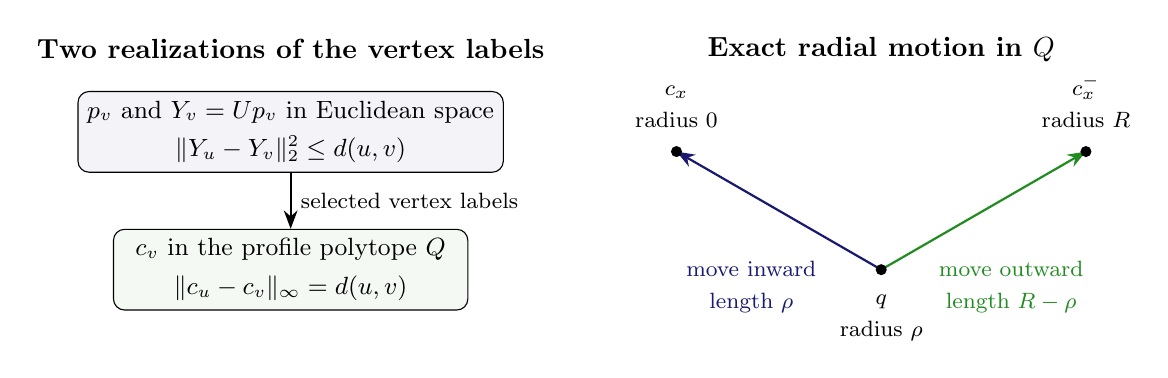
\begin{tikzpicture}[font=\small,>=Stealth]
 \node[font=\bfseries] at (2.7,2.6) {Two realizations of the vertex labels};
 \node[draw,rounded corners,align=center,minimum width=4.5cm,
       fill=MidnightBlue!5] (euclidean) at (2.7,1.55)
       {$p_v$ and $Y_v=Up_v$ in Euclidean space\\[3pt]
        $\norm{Y_u-Y_v}_2^2\le d(u,v)$};
 \node[draw,rounded corners,align=center,minimum width=4.5cm,
       fill=ForestGreen!5] (profiles) at (2.7,-.2)
       {$c_v$ in the profile polytope $Q$\\[3pt]
        $\norm{c_u-c_v}_\infty=d(u,v)$};
 \draw[->,thick] (euclidean) -- node[right,align=left,font=\footnotesize]
       {selected vertex labels} (profiles);
 \node[font=\bfseries] at (10.2,2.6) {Exact radial motion in $Q$};
 \coordinate (center) at (7.6,1.3);
 \coordinate (point) at (10.2,-.2);
 \coordinate (opposite) at (12.8,1.3);
 \draw[->,thick,MidnightBlue] (point) -- (center);
 \draw[->,thick,ForestGreen] (point) -- (opposite);
 \fill (center) circle (2pt);
 \fill (point) circle (2pt);
 \fill (opposite) circle (2pt);
 \node[anchor=south,align=center,font=\footnotesize]
       at (7.6,1.48) {$c_x$\\[2pt]radius $0$};
 \node[anchor=south,align=center,font=\footnotesize]
       at (12.8,1.48) {$c_x^-$\\[2pt]radius $R$};
 \node[anchor=north,align=center,font=\footnotesize,
       text=MidnightBlue] at (8.55,.03)
       {move inward\\[2pt]length $\rho$};
 \node[anchor=north,align=center,font=\footnotesize,
       text=ForestGreen] at (11.85,.03)
       {move outward\\[2pt]length $R-\rho$};
 \node[anchor=north,align=center,font=\footnotesize]
       at (10.2,-.4) {$q$\\[2pt]radius $\rho$};
\end{tikzpicture}
\caption{Spectral packing uses Euclidean points; balls and shells use
the distance-profile realization with the same vertex labels.
The radial paths are schematic: in the ambient norm, distance
traveled along either indicated segment equals change of radius.
The two segments need not form one straight segment in $Q$.}
\label{tg:geometry-figure}
\end{figure}


\subsection{Transferring the bag and charging estimates}

The next lemma extends the bag-selection and shell-charging arguments of
\cite[Propositions B.7, B.8, and B.10]{ThinTreesCompanion} to $Q$.
We retain those constructions and their scalar accounting, but verify
the geometric steps below: their stated cube hypotheses do not cover
all tests in $\mathcal N$.  The two charging alternatives explain the
division into compact and assigned bags.  Compact bags charge disjoint
geometric objects.  Assigned bags may overlap geometrically, provided
their hierarchy labels separate the graph edges used for charging.

Use relative open balls $B(c,\delta)=\{q\in Q:\norm{q-c}<\delta\}$
and strict shells $B(c;a,b)=\{q\in Q:a<\norm{q-c}<b\}$.
An ordinary ball includes its center, whereas a shell with $a=0$
excludes it.  Both are called radial objects.  An ordinary ball
$B(c,b)$ has \emph{numerical} inner radius $a=0$ and width $b$;
a shell has width $b-a$.  All radial tests and width formulas below
apply to both types with these numerical radii, but membership and
intersection always use the actual support.  In particular, an
unchanged ordinary ball keeps its center.  A radial restriction to
$a\le a'<b'\le b$ means replacement by the strict shell
$B(c;a',b')$, even when $a'=0$.  Such a replacement is a subset
of the old support; it is an operation, not an identification of a
ball with a punctured shell.  Proposed intervals of nonpositive
width are discarded.
A \emph{bag} consists of mutually disjoint balls of
a common radius $\delta$, centered at vertex images $c_v$.
It is \emph{$\beta$-compact of type $(\delta,\Delta)$} if it has
at least two balls, its center diameter is at most $\Delta$, and
$\beta\Delta\le\delta|\mathrm{Bag}|$.
It is \emph{$\eta$-assigned to $A$} if
$|\mathrm{Bag}|\ge\eta|O(A)|$ and every ball has a designated center
vertex $u\in A$ with an edge $uv\in O(A)$ of length $d(u,v)<\delta$.
A family has all its balls mutually disjoint and a common radius.
A compact family has a common type $(\delta,\Delta)$.
An assigned family has one bag for each of a set of distinct assigned
nodes. Bags assigned to the same node at one scale may always be
merged: this preserves every witnessing edge, the assignment bound,
and the total mass.  Fix $0<\rho<1$. A sequence of compact
families is $\rho$-geometric when
$\Delta_{i+1}<\rho\delta_i$; a sequence of assigned families is
$\rho$-geometric when $\delta_{i+1}<\rho\delta_i$ and its assigned
nodes are distinct across families.  In either case its mass is
\[
 \mathsf M=\sum_i\delta_i\sum_{\mathrm{Bag}\in\mathcal F_i}
                                      |\mathrm{Bag}|.
\]

\begin{lemma}[Geometric transfer]\label{tg:transfer}
Let $p_v\in\R^{d_{\mathrm E}}$ be points for which
$d(u,v)=\norm{p_u-p_v}_2^2$ is a pseudometric.  Realize $d$ in $Q$
as in \Cref{tg:profiles}.  Let $U:\R^{d_{\mathrm E}}\to\R^{E(G)}$ be a
contraction, change its row signs so
$a_e=\ip{u_e}{p_u-p_v}\ge0$, and set
\[
 d_e=d(u,v),\qquad
 N_A=\frac{(\sum_{e\in O(A)}a_e)^2}{|O(A)|},\qquad
 \mathcal E=\sum_{e\in E(G)}d_e.
\]
The following three assertions hold in $Q$.
\begin{enumerate}[label=(\roman*)]
\item\label{tg:transfer-extract}
Let $T$ be a nonempty set of nodes with $N_A>0$ and
$N_A\ge\alpha\sum_{e\in O(A)}d_e$, where $0<\alpha\le1$.
Define
\begin{align*}
 J&=1+\lceil\log_2(256/\alpha^2)\rceil,&
 C_2&=128J^4,&\sigma&=\alpha/C_2,\\
 L&=2+\lceil\log_2(1/\sigma)\rceil,&
 H_0&=1+\lceil\log_2(24/(\rho\sigma^2))\rceil,&
 C_1&=1024\epsilon^{-2}.
\end{align*}
If $\beta>1$, $0<\epsilon<1/3$, $0<\rho<1$, and
$\sigma^\epsilon\le(48\beta C_1)^{-1}$, there is a
$\rho$-geometric sequence consisting either of $\beta$-compact
families or of $\sigma^{1+2\epsilon}$-assigned families, with
\begin{equation}\label{tg:captured-mass}
 \mathsf M\ge
 \frac{\sigma^\epsilon}{384\beta C_1C_2LH_0}
                  \sum_{A\in T}N_A.
\end{equation}
\item\label{tg:transfer-compact}
For $G$ $k$-edge-connected, a $\rho$-geometric sequence of $\beta$-compact families
with $\rho\le1/12$ and $\beta\ge36$ satisfies
$\mathcal E\ge(k/4)\mathsf M$.
\item\label{tg:transfer-assigned}
For a locally $k$-connected hierarchy, selected nodes satisfying
$|O(A)|\ge k\rho|P(A)|$, and a $\rho$-geometric sequence of
$(24C_3/k)$-assigned families, one has
\begin{equation}\label{tg:assigned-charge}
 \mathcal E\ge\frac{kC_4}{96C_3}\mathsf M
\end{equation}
provided
$C_4\ge3$, $\rho\le(6C_4)^{-1}$, and
$C_3\ge2((C_4+1)+4(C_4+2)^2)$.
\end{enumerate}
\end{lemma}

\begin{proof}
We follow the constructions in Sections B.2--B.4 of
\cite{ThinTreesCompanion}, keeping their scale choices and scalar
potentials.  All balls, shells, and intersections now lie in the
continuous polytope $Q$.  New shells inherit vertex centers, so
\Cref{tg:affine-radius} remains available.  We first obtain the bags,
then explain how each of the two charging constructions operates in
this realization.

\emph{Extraction and the spectral step.}
The two truncations and homogeneity arguments in
\cite[Section B.2.2]{ThinTreesCompanion} use only
$a_e^2\le d_e$, nonnegative boundary sums, and multiplicity at most
two.  They select nonempty subsets $O'(A)\subseteq O(A)$ retaining
a fixed fraction of each squared boundary sum, and group the nodes
so that both positive quantities $a_e^2$ and $d_e$ vary by a factor
less than four within $F=\bigcup_AO'(A)$.  For one such group put
$N=\sum_A|O(A)|$, $N'=|F|$,
$c_1=\min_{e\in F}a_e^2$, and $c_2=\max_{e\in F}d_e$.
The truncation and grouping estimates give $c_1N'\ge\sigma Nc_2$.
For the Euclidean points $Y_v=Up_v$ and
$\widetilde\alpha=\sigma N/N'$ this implies
\[
 (\E_{e\in F}a_e)^2\ge c_1
 \ge\widetilde\alpha c_2
 \ge\widetilde\alpha\E_{e\in F}\norm{Y_u-Y_v}_2^2.
\]
This is the exact hypothesis of the Euclidean spectral-packing
Lemma B.3 of \cite{ThinTreesCompanion}; that lemma places no binary
restriction on its points.  Its selected centers have squared
Euclidean separation at least $4r$.  Since
\begin{equation}\label{tg:spectral-to-metric}
 \norm{Y_u-Y_v}_2^2\le d(u,v)=\norm{c_u-c_v}_\infty,
\end{equation}
the corresponding $Q$-balls of radius $r$ are disjoint.  If $b_0$
is their number, the spectral lemma gives
$b_0r\ge\widetilde\alpha^\epsilon c_1N'/C_1$.  Shrink their common
radius to $\delta$ defined by
$b_0\delta=\widetilde\alpha^\epsilon c_1N'/C_1$.
Only the selected vertex labels pass from the Euclidean geometry
to $Q$; a map on intermediate points is unnecessary.

The rest of the one-family construction uses a maximal disjoint
collection of balls of radius $D=\max\{\delta,2c_2\}$, centered at
images $c_u$ for which $u\in A$ and $uv\in O'(A)$ for some $A$.
Maximality puts every candidate center within $2D$ of a selected
center: intersection of two relative balls implies this distance
bound by the triangle inequality.  Every endpoint center is within
$c_2$ of an assigned endpoint, hence within $3D$ of a selected center.
Grouping by those centers gives diameter at most $6D$ in the compact
case.  In the assigned case the witnessing edge has length
at most $c_2<D$.  The cardinality estimates of
\cite[Lemma B.6]{ThinTreesCompanion} give compactness, assignment
strength, and radius range
$[\sigma c_1,12c_1/\sigma]$.  Its final grouping by dyadic size and
then by residue class modulo $H_0$ is numerical: each scale lies
between $\sigma2^j$ and $24\,2^j/\sigma$, so scales in the same
residue class meet the stated geometric separation.  The losses
$C_2$, $L$, $2H_0$, and $192\beta C_1/\sigma^\epsilon$ are exactly
those in \Cref{tg:captured-mass}.  This proves (i).

\emph{Length charging and compact radial objects.}
The resource charged by both arguments is one fixed straight
segment $[c_u,c_v]$ of length $d_e$ for each graph edge, retaining
parallel edges as separate resources.  For a radial object with numerical radii
$a<b$, its clamped radial function is
$f(q)=\min\{b,\max\{a,\norm{q-c}\}\}$.
It is $1$-Lipschitz and piecewise affine on each edge segment.
If the object has vertex witnesses at radius at most $a$ and at
least $b$, all its intermediate radial cuts are nontrivial.
Consequently
\[
 k(b-a)\le\int_a^b|\delta_G\{v:\norm{c_v-c}<t\}|\,dt
 =\sum_{uv\in E(G)}|f(c_u)-f(c_v)|.
\]
For disjoint radial objects, subdivide an edge segment at the finitely many
breakpoints of these functions.  At most one clamped function is
nonconstant on each open subsegment, and its variation is bounded
by that subsegment's length.  The total charge is therefore at most
$d_e$, including edges along a boundary or of zero length.  This
proves the length bound of \cite[Lemma B.9]{ThinTreesCompanion} in $Q$.
For an ordinary ball, nonconstant portions of the clamped function
lie at strictly positive radius.  Its center contributes no charged
length, but remains part of the ball in membership tests.

For compact bags, process the families in decreasing order of radius,
as in \cite[Proposition B.8]{ThinTreesCompanion}.  An input ball inserted
at the current scale is called fresh and is left intact until the
next scale; all other live objects are called old.  Thus a fresh
ordinary ball becomes an old ordinary ball at the next scale unless
a subsequent operation restricts it.  Disjoint
equal-radius balls have centers separated by at least $2\delta$,
since their midpoint belongs to $Q$.  For any live object with center
$c$ and numerical radii $a,b$, call $B(c_u,\delta)$ interior when
\[
 a+\delta+\Delta\le\norm{c_u-c}\le b-\delta-\Delta.
\]
This conservative two-sided test also applies when the object is
an ordinary ball, with $a=0$.  If one ball of a compact bag is
interior, its containing object is old, since fresh balls and
unprocessed balls belong to the same disjoint family.  All bag centers
have radial values in an interval $[l,u]\subseteq[a+\delta,b-\delta]$
of width at most $\Delta$.  Replacing the old object by the strict
shells with intervals $(a,l-\delta)$ and $(u+\delta,b)$ leaves room
for all the new balls, including when the old object was ordinary.
The extremal centers supply the new outer and inner witnesses;
the previous witnesses supply the other two.  Every inserted ball
has its own center and a different bag center as witnesses.
All supports are disjoint by $1$-Lipschitzness of radius.
When no interior bag remains, shrinking each old interval at both
ends by $2\delta+\Delta$ separates it from every remaining ball.
Indeed, failure at the lower margin puts the entire candidate at
radius less than $a+2\delta+\Delta$, and failure at the upper
margin puts it beyond $b-2\delta-\Delta$.  This includes candidates
near the center of an old ordinary ball: the shrink removes that
center neighborhood.  Witnesses are preserved because the inner
radius increases and the outer radius decreases; an inner witness
need not belong to the remaining strict shell.
The capacities $[w-6\Delta_i]_+$ for all old objects and
$\delta_i-6\Delta_{i+1}$ for fresh balls depend only on widths and
the inequalities $2\delta_i\le\Delta_i$,
$6\Delta_{i+1}\le\delta_i/2$, and
$|\mathrm{Bag}|\delta_i\ge36\Delta_i$, all verified here.
The split loses numerical width $(u-l)+2\delta$, and the shrink
loses $2(2\delta+\Delta)$, with the same positive-part accounting
when a residual is discarded.  Removing the center alone adds no
width loss.  A retained fresh ball has the same capacity after
becoming old.  Thus the split and scale-transition inequalities in
the cited proof retain at least one quarter of the input mass as
final radial-object width.
Applying the preceding length bound proves (ii).

\emph{Assigned labels, pruning, and path charging.}
Assigned bags require the labeled records of
\cite[Section B.4.1]{ThinTreesCompanion}.  We give their definitions
because geometric overlap is allowed.  Write $\mathcal T[A]$ for
the hierarchy subtree rooted at $A$, identifying its leaves with the
vertices in $A$.  A record $H$ has an ordinary ball or shell as its
support, an owner $A_H$, a set $\mathcal P_H$ of strict descendants
of $A_H$, and optionally one avoided strict descendant $D_H$.
Define its conflict domain and leaf set by
\[
 C(H)=\mathcal T[A_H]\setminus
 \left(\bigcup_{P\in\mathcal P_H}\mathcal T[P]
       \ \cup\ \mathcal T[D_H]\right),
 \qquad L(H)=C(H)\cap V,
\]
omitting the final subtree when there is no avoided label.
The record is called avoiding precisely when $D_H$ is present.
For center $c$ and numerical radii $a<b$, validity means:
\begin{enumerate}[label=(\alph*)]
\item the labels have the stated form, so $A_H\in C(H)$;
\item both endpoints of every edge of $\delta_G(P)$,
      for every $P\in\mathcal P_H$, have radius at least $b$ from $c$;
\item some $u\in L(H)$ has radius at most $a$ and starts at least
      $k/4$ edge-disjoint paths to vertices of radius at least $b$.
      These paths lie in $G[A_H]$, or in $G[A_H\setminus D_H]$
      for an avoiding record;
\item geometrically intersecting records have disjoint conflict domains.
\end{enumerate}
The initial paths in (c) need not avoid the predecessor subtrees
in $\mathcal P_H$; condition (b) will remove those subtrees from
the portions used for charging.  Its inner witness is a graph
vertex in $L(H)$, not necessarily a point of the support: for a
strict shell it can lie on or inside the excluded inner boundary.

For a node $A$ assigned at scale $\delta_i$, its predecessors are
the strict descendants assigned at earlier, larger scales.  An input
ball is noninsertable if it contains an endpoint of a boundary edge
of any predecessor.  Otherwise give it owner $A$, no avoided label,
and excluded set equal to the predecessors.

At one scale, disjoint center-inclusive balls contain at most
$2|P(A)|$ endpoint vertices of $P(A)$.  Thus a predecessor $A$,
whose own scale is $\delta_i$, deletes mass at most
$4\rho\delta_i|P(A)|$, which the boundary ratio and
assignment bound pay as in the source's Lemma B.13.  Deleting
noninsertable balls and bags losing more than half their balls
retains mass at least $\mathsf M/2$ and assignment at least
$12C_3/k$.  Insertability puts the designated center vertex in
its conflict domain: otherwise its witnessing edge in $O(A)$
would be a forbidden predecessor-boundary edge whose endpoint
lies in the ball.  Another ball of the bag supplies an outer
vertex; local connectivity supplies the required paths.
The retained bag has more than one ball, since
$|O(A)|\ge k$ and its assignment is at least $12C_3/k$.
Thus the resulting input records satisfy (a)--(c), including when
distinct vertices have coincident images.

For a valid collection, stop each witnessing graph path at its
first outer vertex.  It cannot enter an excluded predecessor
subtree earlier, because the entering edge would have an endpoint
inside the outer radius.  On the resulting continuous path keep
the portion from the last inner-radius point to the first
outer-radius point.  Its length is at least the record's numerical
width by $1$-Lipschitzness.  Apart from endpoints it lies in
$a<\norm{q-c}<b$, which is contained in either type of support.
For an ordinary ball $a=0$ and the center carries no charged length.
Paths within one record are edge-disjoint.
Both endpoints of every edge in a stopped path belong to $L(H)$:
an entrance into an excluded subtree, even at the stopping vertex,
would have a preceding endpoint inside the outer radius, contradicting
(b).  Two records charging the same graph edge therefore have intersecting
conflict domains, so (d) makes their actual supports disjoint and
they charge disjoint open portions of that edge.  This proves
the source's Lemma B.14 in $Q$, at rate $k/4$.

It remains to construct a valid arrangement with enough total width.
Start with the empty arrangement and process scales in decreasing
order and, within each scale, bags in
increasing depth of their assigned nodes.  As in the compact
construction, original balls inserted during the current phase are
fresh and remain intact until the next phase; all other records are
old.  A candidate
$J=B(c_u,\delta_i)$ is interior to a current record
$H$ with center $c$ and numerical radii $a,b$ when
\[
 C(J)\cap C(H)\ne\varnothing,
 \qquad a+C_3\delta_i<\norm{c_u-c}<b-C_3\delta_i.
\]
A candidate interior to no current record is called a border
candidate.  In particular old ordinary balls participate in this
test with $a=0$, including its lower margin.  A record containing an
interior candidate has width greater than $2C_3\delta_i$, so it
cannot be a fresh ball of width $\delta_i$.  An interior candidate is
contained in $H$.  The processing order implies that the owner of
any conflicting current record is an ancestor of the candidate's
owner $A$, and that $A\in C(H)$.  Two conflicting records therefore
cannot both contain this candidate, by (d).  The strict concentric
restrictions defined above retain (a)--(c) with the old labels:
the old inner witness still has radius at most the new inner
radius, and the old paths still reach the smaller outer radius.
This remains true when an ordinary ball is replaced by a shell
and its center witness no longer lies in the support.
Restricting both support and conflict domain
preserves (d).  Discard any proposed radial interval of nonpositive
width.  Such restrictions cannot turn a border candidate
into an interior candidate.  These are the order and inheritance
properties of \cite[Lemmas B.17--B.20]{ThinTreesCompanion}.

\emph{Meeting a record and carving its interior.}
The following consequence of \Cref{tg:profiles} identifies the record
affected by a carving operation.  If a live record $H$ with center
$c$ and numerical radii $r_1<r_2$, and a vertex center $z$, satisfy
\[
 r_1-\delta<\norm{z-c}<r_2+\delta,
\]
then $B(z,\delta)$ meets the actual support of $H$.
Choose a radius in $(r_1,r_2)$
less than $\delta$ away from $\norm{z-c}$ and use the exact inward
or outward motion to reach it.  Its traveled distance is less than
$\delta$.  There is no radius-range obstruction: condition (c)
provides an outer vertex witness, so $r_2\le\operatorname{diam}(d)<R$.
For an ordinary ball $r_1=0$; the chosen radius is positive and
belongs to that ball, even when $z=c$ and outward motion is needed.
This replaces motion toward the binary center or its opposite cube
vertex in \cite[Section B.4.3]{ThinTreesCompanion}.

At scale $\delta$, process the interior candidates of a bag assigned
to $A$ while at least half its original balls remain interior and
untreated.  Candidates that cease to be interior are kept as border
candidates.  Carving an avoiding shell around an interior candidate
replaces its radial interval $(r_1,r_2)$ by
$(r_1,q-\delta)$ and $(q+\delta,r_2)$, and inserts the candidate.
Here $q$ is its center's radius from the shell center.
Every avoiding record is indeed a strict shell: input records are
nonavoiding, only the central shell $H_4$ below introduces an
avoided label, and later restrictions are strict shells.
Radial Lipschitzness gives disjointness; witnesses and labels
survive in the restrictions.  If no remaining interior candidate
belongs to an avoiding shell, the other two operations first split
$G[A^*\setminus A]$ into $j\le2|O(A)|/k$ induced subgraphs
that are $k/4$-edge-connected.  This count follows by successive
cuts smaller than $k/4$ and the $k$-connectivity of $G[A^*]$;
it is independent of the embedding.  Assignment and the
half-bag loop condition give one piece adjacent along edges of
length less than $\delta$ to at least $3C_3$ candidate centers.
Radial coordinates of these neighbors differ by less than
$\delta$ from those of their candidate centers.

Choose a nonavoiding record $H$ containing one of those candidates
in its interior, with center $c$ and numerical radii $r_1,r_2$,
and write $\varrho(v)=\norm{c_v-c}$.  It may be an old ordinary
ball, in which case $r_1=0$.
Let $[a,b]\subseteq[r_1,r_2]$ be the radial range of the neighbors
in the selected piece, clipped to this numerical interval.  Select for treatment
the $m$ still-interior candidates whose centers have radii in
$(a-\delta,b+\delta)$.  Each meets the chosen record by the preceding
exact-motion argument.  All candidates of the bag have the same
labels, so each has conflict domain meeting $C(H)$.  If such a
candidate is interior to another record $H'$, its entire ball lies
in $H'$, so $H$ and $H'$ intersect.  The processing-order property
puts its owner $A$ in both conflict domains, contrary to (d).
Thus every selected candidate is interior to $H$ itself.
The radial count in the cited proof gives
$m\ge3(C_3-1)$ in the dense case below and
$b-a\ge(C_3-1)\delta$ in the sparse case.  It uses only the
$3C_3$ adjacent centers, their interior margins, and the fact that
neighbor radii differ by less than $\delta$.

For the dense case, with $m\delta>3(b-a)$, retain intervals
$(r_1,a-2\delta)$ and $(b+2\delta,r_2)$ and insert the $m$ balls.
The expanded radial interval and Lipschitzness give every required
separation.  For the sparse case $m\delta\le3(b-a)$, retain
$(r_1,a)$ and $(b,r_2)$ and create the central shells
$H_3=B(c;a+\delta,b-\delta)$ and $H_4=B(c;a,b)$.
Give $H_3$ owner $A$, no avoided label, and the old excluded nodes
strictly below $A$.  Give $H_4$ the old owner and excluded set,
and avoided label $A$.  Their domains are respectively
$C(H)\cap\mathcal T[A]$ and $C(H)\setminus\mathcal T[A]$.
The old owner is a strict ancestor of $A$.  An original ball with
owner $A$ cannot come from an earlier scale, since assigned nodes
are distinct across families; at the current scale it is disjoint
from every unprocessed candidate.  A synthetic shell with owner
$A$ can only have been created while processing this same bag.
It has already treated every then-interior candidate in its expanded
interval; later restrictions only reduce its support, and border
candidates never become interior.  Hence neither an original ball
nor a synthetic shell with owner $A$ can be the chosen record.
Thus both new labels have the required form.
For the changed-label path witnesses, extremal neighbors
$v_1,v_2$ in the selected piece and their adjacent candidates
$u_1,u_2\in A$ satisfy
\[
 \varrho(v_1)\le a,\quad \varrho(v_2)\ge b,\qquad
 \varrho(u_1)<a+\delta,\quad \varrho(u_2)>b-\delta.
\]
Connectivity of $G[A]$ supplies $k$ paths for the inner central
shell; connectivity of the selected piece supplies at least
$k/4$ paths for the avoiding shell.  Their initial vertices
avoid excluded subtrees: membership in one would make the
short edge $u_1v_1$ an excluded boundary edge with an endpoint
inside the old outer radius, or make that excluded subtree an
ancestor of $A$, contradicting $A$'s conflict membership.
The sparse-case width bound gives $a+\delta<b\le r_2$, so the
initial vertices used here lie strictly inside the old outer radius.
This verifies (c) for both new labels; (b) follows from the smaller
outer radii and excluded sets.  Other records inherit separation by support and
conflict-domain inclusion.  Remaining interior candidates have centers
outside $(a-\delta,b+\delta)$, so miss both central shells.
If $a=0$, $H_4$ excludes its center but may still use $v_1$ at
radius zero as its inner witness, as condition (c) permits.

\emph{The scalar accounting and the phase transition.}
The potentials in Section B.4.3 are
$\delta_i-C_4\delta_{i+1}$ for fresh balls,
$[w-C_4\delta_i]_+$ for other nonavoiding records, and the
latter divided by $2(C_4+2)$ for avoiding records.
An original ball becomes old when its phase ends and then uses the
second formula with width equal to its radius; if retained unchanged,
it still has its center-inclusive support.  These functions use the
same numerical widths and radii in $Q$.  The three
replacements have formal width losses $2\delta$ across the two avoiding residual
shells in the first operation, $(b-a)+4\delta$ across the two
nonavoiding residual shells in the second, and $2\delta$ across
the three nonavoiding pieces in the third.  Its numerical
inequalities preserve old credit and supply
$C_4\delta/(6C_3)$ per treated candidate, counting sparse-case
candidates as treated even though their balls are not inserted.
Finally, Section B.4.4 either retains every record when the gain
from changing scale supplies the required border credit, or shrinks
every old object, including old ordinary balls, at both ends by
$(C_3+1)\delta_i$ and inserts remaining border balls when the
gain is insufficient.  For a conflicting old object, border status
means the candidate center has radius at most $a+C_3\delta_i$
or at least $b-C_3\delta_i$.  Its whole ball therefore lies below
the new inner radius or above the new outer radius, respectively.
This proves separation also at the center of an old ordinary ball;
fresh balls are disjoint within the current family.  Restrictions
retain witnesses.  Each old width decreases by
$2(C_3+1)\delta_i$, unless the object is discarded, while the
potential threshold decreases from $C_4\delta_i$ to
$C_4\delta_{i+1}$.  These are the same changes for a ball and a
shell.  The source's width
calculation bounds the lost potential by half the inserted
mass, leaving at least $C_4/(6C_3)$ of each border ball's radius
for its node.  The half-bag stopping rule leaves final width at
least $C_4/(12C_3)$ times the retained mass.  Combined with the
pruning factor $1/2$ and the path-charging rate $k/4$, this is
exactly \Cref{tg:assigned-charge}.

Thus the inherited constructions give (i)--(iii), with the same
scalar losses and with every length charge measured by
$\mathcal E=\sum_e d_e$ in the profile realization.
\end{proof}

\subsection{Choosing parameters and responding to a partition chain}

\begin{proof}[Proof of \Cref{thm:tg-hierarchy}]
If $\mathcal M$ is empty, a sufficiently small positive centered
identity satisfies \Cref{tg:shortcut}.  Otherwise use
\Cref{tg:dual}.  Fix one of its embeddings and row-orthonormal
systems, with $\mathcal E>0$, and set
\[
 \alpha=h^{-4/5},\qquad \epsilon=1/10,\qquad
 \beta=36,\qquad \rho=(2h^2)^{-1},\qquad
 C_3=10^4,\qquad C_4=3.
\]
Let $T$ consist of the marked nodes with positive $N_A$ and
$N_A\ge\alpha\sum_{e\in O(A)}d_e$.
Boundary multiplicity at most two gives
\begin{equation}\label{tg:good-nodes}
 \sum_{A\in\mathcal M\setminus T}N_A\le2\alpha\mathcal E.
\end{equation}
If $T$ is nonempty, apply \Cref{tg:transfer}(i).
Its parameters obey
\[
 C_2=O((1+\log h)^4),\quad L,H_0=O(1+\log h),\quad
 \sigma=h^{-4/5}/C_2.
\]
The smallness condition holds for all sufficiently large absolute
$h$.  So does the assignment requirement, because
\[
 h\sigma^{1+2\epsilon}
 =h^{1/25}/C_2^{6/5}\longrightarrow\infty,
 \qquad \sigma^{1+2\epsilon}\ge24C_3/h.
\]
The marked-node condition implies
$|O(A)|\ge|P(A)|/h\ge h\rho|P(A)|$.
For large $h$, $\rho\le1/18$; also
$10^4\ge2(4+4\cdot25)=208$.
Both charging conclusions of \Cref{tg:transfer} therefore apply,
according to the family type, and give the common bound
\[
 \mathcal E\ge c_*h\mathsf M,
 \qquad c_*=\frac{C_4}{96C_3}=\frac{1}{320000}.
\]
Together with \Cref{tg:captured-mass}, this yields
\[
 \frac{\sum_{A\in T}N_A}{\mathcal E}
 \le \frac{384\beta C_1C_2LH_0}{c_*h\sigma^\epsilon}
 =O\bigl(h^{-23/25}(1+\log h)^7\bigr).
\]
Indeed $\sigma^\epsilon=h^{-2/25}C_2^{-1/10}$, so the exact
logarithmic exponent before rounding upward is $32/5<7$.
Including \Cref{tg:good-nodes}, or using it alone when $T$ is empty,
every ratio in \Cref{tg:dual-ratio} is at most
\begin{equation}\label{tg:final-ratio}
 2h^{-4/5}+O\bigl(h^{-23/25}(1+\log h)^7\bigr)
 =o(h^{-31/40}).
\end{equation}
The exponent margins are $1/40$ and $29/200$, respectively.
Increase $h_0$ so the bound is at most $h^{-31/40}/2$.
Then $p_*\le h^{-31/40}/2$, and the defining property of the
infimum supplies a feasible positive definite $D$ with marked
averages less than $h^{-31/40}$.  No attainment assumption is used.
\end{proof}

For a fixed connected ambient graph $H$, define
\begin{equation}\label{tg:compact-domain}
 \mathcal K_H=\{X\succeq L_H:
       \ip{X}{Z}\le3\ip{L_H}{Z}\quad(Z\in\mathcal N)\}.
\end{equation}
This set is nonempty, convex, and compact.  It contains $L_H$;
closedness is immediate, and the test $\Id_{\mathsf E}$ bounds
$\tr X$ by $3\tr L_H$.  For $X\succ0$ write
$R_X(e)=b_e^TX^{-1}b_e$.  Two elementary identities used below are
\begin{equation}\label{tg:resistance-order}
 X\succeq D\succ0\ \Longrightarrow\ R_X(e)\le R_D(e),
 \qquad
 X\succeq t b_eb_e^T\ \Longleftrightarrow\ tR_X(e)\le1
 \quad(t>0).
\end{equation}
The first follows by inverse order, and the second by congruence
with $X^{-1/2}$ and the single nonzero eigenvalue of a rank-one matrix.

\begin{proposition}[Simultaneous response]\label{prop:tg-response}
Let $H$ be connected and let $G\subseteq H$ be a spanning subgraph.
Let $r$ be a sufficiently large integer, put $h=\lfloor r/2\rfloor$,
and suppose $G$ and the subgraphs induced by all parts of a nested
sequence of partitions are $h$-edge-connected, with the singleton
condition vacuous.  If $0<s\le r^{1/4}$, there is $Y\in\mathcal K_H$
such that, at every partition $\mathcal P$ in the sequence, all but
at most $r^{-1/3}|E_G(\mathcal P)|$ crossing edges satisfy
\begin{equation}\label{tg:response-edge}
 Y\succeq6s\,b_eb_e^T.
\end{equation}
Here $E_G(\mathcal P)$ denotes the edges whose endpoints lie in
different parts of $\mathcal P$.
\end{proposition}

\begin{proof}
Use the dyadic assembly of \cite[Lemma 4.2]{ThinTreesCompanion}, with
the hierarchy estimate and threshold just proved; we give the
counting argument to specify both constants.  In each occupied bin
$2^a\le |E_G(\mathcal P)|<2^{a+1}$ choose the finest partition.
List these representatives from fine to coarse as
$\mathcal P_0,\ldots,\mathcal P_{\ell-1}$, and append
$\mathcal P_\ell=\{V\}$.  Put
$B_i=E_G(\mathcal P_i)$ and $M_i=|B_i|$, with $M_\ell=0$.
Distinct parts of these representative partitions, together with $V$ and singleton leaves,
form a locally $h$-connected hierarchy.  Mark precisely the nodes
with $|O(A)|\ge|P(A)|/h$, and take $D$ from
\Cref{thm:tg-hierarchy}.  Then
\[
 Y=L_H+D\in\mathcal K_H,
\]
because $Y\succeq L_H$ and, for every $Z\in\mathcal N$,
$\ip{Y}{Z}\le\ip{L_H+L_G}{Z}\le2\ip{L_H}{Z}$.

At transition $j$ to $j+1$, the parent of each changing part is
the part of $\mathcal P_{j+1}$ containing it.  Every disappearing
edge in $B_j\setminus B_{j+1}$ belongs to parent boundaries of
changing parts, whose total full-boundary size is at most $2M_j$.
Unmarked parts therefore cover at most $2M_j/h$ such edges.
For marked parts, \Cref{tg:resistance-order} and Markov's
inequality give
\[
 |\{e\in O(A):R_Y(e)>1/(6s)\}|
 \le6s\,h^{-31/40}|O(A)|.
\]
Thus at most $2(h^{-1}+6s h^{-31/40})M_j$ disappearing edges
fail \Cref{tg:response-edge}.  Double counting only increases
this upper bound.

There is at most one representative per dyadic bin, and its bin
index strictly decreases.  Hence
$\sum_{j=i}^{\ell-1}M_j<4M_i$.  Each edge of $B_i$ disappears
at exactly one subsequent transition, so its bad-edge count is
at most $8(h^{-1}+6s h^{-31/40})M_i$.
For a skipped partition with positive crossing count $M$, its
representative is finer and has $M_i<2M$.  Consequently its
bad-edge count is at most
\begin{equation}\label{tg:response-fraction}
 16(h^{-1}+6s h^{-31/40})M
 =O(r^{-1}+r^{-21/40})M\le r^{-1/3}M
\end{equation}
for a sufficiently large absolute cutoff.  The final inequality
uses $21/40-1/3=23/120>0$.  Partitions with no crossing edges
need no estimate.  One matrix $Y$ therefore works for the whole
nested sequence.
\end{proof}

\section{Constructive shortcut extraction}
\label{sec:ta-algorithm}

We now turn the simultaneous response of \Cref{prop:tg-response} into an
algorithm. Throughout this section, an explicit multigraph has distinct
labels for its parallel edges, and loops are discarded. Write
$E_H(\mathcal P)$ for the edges crossing a partition $\mathcal P$ of the
vertex set. Matrices act on $\one^\perp$, with its inherited Euclidean
inner product. We retain the cone $\mathcal N$ and compact convex set
$\mathcal K_H$ from the preceding section:
\begin{equation}
 \mathcal K_H=\{X\succeq L_H:
       X\mathbin\bullet Z\le3L_H\mathbin\bullet Z\quad(Z\in\mathcal N)\}.
 \label{eq:ta-K}
\end{equation}
Here $A\mathbin\bullet Z=\tr(AZ)$ always means the inherited trace, even
when rational, nonorthonormal coordinates are used for computation.



The construction follows the packing-preserving sparsification strategy
of \cite{ThinTreesCompanion}. Convex continuation produces a rational
shortcut together with a large integer packing supported on its
low-resistance edges. Nonnegative capacities permit partition uncrossing;
the nearly tight partitions then have highly connected parts, which is
precisely the input required by the simultaneous geometric response.

\subsection{A ramp of packing capacities}

We use two standard algorithmic inputs in precise forms. The
Nash--Williams--Tutte tree-packing theorem
\cite{NashWilliams1961,Tutte1961} says that a multigraph contains $q$ edge-disjoint
spanning trees if and only if
\begin{equation}
 |E_H(\mathcal P)|\ge q(|\mathcal P|-1)
                \quad\hbox{for every partition }\mathcal P;
 \label{eq:ta-integer-packing}
\end{equation}
see \cite[Theorem~1]{Kaiser2012}. A maximum union of $q$ graphic matroids
can be constructed by matroid partition, originating with Edmonds
\cite{Edmonds1968}; we use the polynomial-time independence-oracle
algorithm of \cite[Theorem~14]{Terao2023}. The algorithm
returns disjoint forests of maximum total cardinality. Their total size
is $q(n-1)$ exactly when all $q$ forests are spanning trees. Acyclicity
is a polynomial-time independence test, including for parallel edges.
We reject $q(n-1)>m$ before invoking this procedure; thus the number of
matroid copies is polynomial for an explicit graph.

\begin{proposition}[Constructive shortcut extraction]
\label{prop:ta-extraction}
There are absolute constants $A$ and $r_0$ such that the following holds.
If an explicit multigraph $H$ on at least two vertices contains $r\ge r_0$
edge-disjoint spanning trees, one can deterministically compute a rational
$X\in\mathcal K_H$ and at least
\[
                 (1-Ar^{-1/16})r
\]
edge-disjoint spanning trees, every edge $e$ of which satisfies
$b_e^TX^{-1}b_e\le r^{-1/4}$. The running time and output encoding length
are polynomial in $|V(H)|+|E(H)|$.
\end{proposition}

Fix such an $H$, put $m=|E(H)|$, and set
\begin{equation}
 \kappa=\frac1{m+1},\qquad t=\frac\kappa{32},\qquad
 r^{-1/8}\le g\le2r^{-1/8},
 \label{eq:ta-parameters}
\end{equation}
where $g$ is dyadic. Comparing eighth powers computes $g$ exactly with
$O(\log r)$ bits. At a parameter $s>0$ and matrix $X\in\mathcal K_H$, define
\begin{equation}
 R_e(X)=b_e^TX^{-1}b_e,\qquad
 p_e=\min\{2,(sR_e(X))^{-1}\},\qquad
 u_e=\max\{0,p_e-1\}.
 \label{eq:ta-ramp}
\end{equation}
The maintained invariant is
\begin{equation}
 \sum_{e\in E_H(\mathcal P)}(u_e+\kappa)
       \ge Q(|\mathcal P|-1)\qquad\hbox{for every }\mathcal P.
 \label{eq:ta-invariant}
\end{equation}
Initially take $s=1/2$, $X=L_H$, and $Q=r$. Since
$L_H\succeq b_eb_e^T$, each $R_e(L_H)\le1$, so $u_e=1$ and the initial
invariant follows from the given packing.

One step replaces
\begin{equation}
 s^+=(1+t)s,\qquad X^+=(1-t)X+tY,\qquad Q^+=Q-2grt,
 \label{eq:ta-step}
\end{equation}
where $Y\in\mathcal K_H$ is to be found. Steps are performed while
$s^4<r$, an exact rational comparison. The final step may overshoot
$r^{1/4}$; every response is invoked at an old parameter
$s\le r^{1/4}$. There are
$O(t^{-1}(1+\log r))$ steps, since $\log(1+t)\ge t/2$. Consequently
\begin{equation}
 r\ge Q\ge r\bigl(1-O(r^{-1/8}(1+\log r))\bigr)\ge3r/4
 \label{eq:ta-target-bound}
\end{equation}
after increasing the absolute cutoff $r_0$.

Let $G$ be the active subgraph with edges $u_e>0$. Choose variables
$0\le y_e\le1$ for $e\in E(G)$ and impose
\begin{equation}
                 Y\succeq6s y_e b_eb_e^T.
 \label{eq:ta-response-LMI}
\end{equation}
For these variables define concave lower capacities on all edges of $H$:
\begin{equation}
 a_e(y)=
 \begin{cases}
 \kappa+\min\{1,u_e+t(5y_e-4)\},&e\in E(G),\\
 \kappa,&e\notin E(G).
 \end{cases}
 \label{eq:ta-lower-capacity}
\end{equation}
They are nonnegative, in fact $a_e\ge\kappa-4t=7\kappa/8$.
This small baseline will also make the uncrossing argument valid.

To check the lower bound, recall that $X\succeq\alpha b b^T$ is
equivalent to $\alpha\le(b^TX^{-1}b)^{-1}$ for $X\succ0$.
Thus $X\succeq sp_e b_eb_e^T$, and \Cref{eq:ta-response-LMI} gives
\[
 \frac1{s^+R_e(X^+)}\ge
       \frac{(1-t)p_e+6ty_e}{1+t}
       \ge p_e+t(5y_e-4).
\]
Indeed the numerator of the difference in the last inequality, divided
by $t$, is $(1-5t)y_e+4+4t-2p_e\ge0$, since $p_e\le2$ and $t<1/5$.
Taking the ramp at $s^+,X^+$, including both its upper cap and its lower
truncation, proves
\begin{equation}
                         u_e^++\kappa\ge a_e(y).
 \label{eq:ta-ramp-lower}
\end{equation}
Off $G$ this follows just from $u_e^+\ge0$.

\begin{lemma}[A feasible continuation response]
\label{lem:ta-continuation}
Under \Cref{eq:ta-invariant,eq:ta-target-bound}, with
$s\le r^{1/4}$, there exist $Y\in\mathcal K_H$ and $y$ satisfying
\Cref{eq:ta-response-LMI} and
\begin{equation}
 \sum_{e\in E_H(\mathcal P)}a_e(y)
       \ge (Q-grt)(|\mathcal P|-1)
                  \qquad\hbox{for every }\mathcal P.
 \label{eq:ta-strong-target}
\end{equation}
\end{lemma}

\begin{proof}
Let $\mathcal C$ be the compact convex set of admissible $(Y,y)$ before
the partition inequalities are imposed. It is nonempty: take $Y=L_H$
and $y=0$. Put $q=Q-grt>0$ and let
\[
 S_{\mathcal P}(y)=\sum_{e\in E_H(\mathcal P)}a_e(y)
                         -q(|\mathcal P|-1).
\]
Each slack is continuous and concave. Its vector image need not be
convex, but the downward set
\[
 \mathcal D=\{v:\ v_{\mathcal P}\le S_{\mathcal P}(y)
                 \text{ for some }(Y,y)\in\mathcal C\}
\]
is convex and closed. Convexity follows coordinatewise from concavity;
closedness follows by taking a convergent subsequence of witnesses in
$\mathcal C$. The set $\mathcal D$ is unbounded downward. If it does not
meet the nonnegative orthant, its distance from that orthant is positive:
the norm of the negative part of $S(y)$ has a positive minimum on the
compact set $\mathcal C$, and passing downward cannot reduce that norm.
Separation therefore supplies nonnegative weights $w_{\mathcal P}$,
normalized to sum to one, for which
\begin{equation}
 F(w):=\max_{(Y,y)\in\mathcal C}
                \sum_{\mathcal P}w_{\mathcal P}S_{\mathcal P}(y)<0.
 \label{eq:ta-separated}
\end{equation}

There are finitely many partitions. Hence $F$ is continuous on their
probability simplex and has a minimizer. Among minimizers choose one
maximizing $\sum_{\mathcal P}w_{\mathcal P}|\mathcal P|^2$.
Its support is a chain under refinement. To prove this, suppose
incomparable $\mathcal P,\mathcal Q$ have positive mass. Move equal mass
from them to their common refinement $\mathcal P\wedge\mathcal Q$ and
finest common coarsening $\mathcal P\vee\mathcal Q$. For each edge,
\[
 \one_{E_H(\mathcal P\wedge\mathcal Q)}+
 \one_{E_H(\mathcal P\vee\mathcal Q)}
 \le \one_{E_H(\mathcal P)}+\one_{E_H(\mathcal Q)}.
\]
Moreover,
\[
 |\mathcal P\wedge\mathcal Q|+|\mathcal P\vee\mathcal Q|
       \ge |\mathcal P|+|\mathcal Q|.
\]
For the second inequality, form the bipartite graph whose vertices are
parts of $\mathcal P$ and $\mathcal Q$ and whose edges are their nonempty
intersections. Its edges count refinement parts, and its connected
components count coarsening parts; edges plus components are at least
vertices. Since $a_e\ge0$ and $q>0$, uncrossing decreases the weighted
slack for every $(Y,y)$, hence cannot increase $F$.
Writing $a=|\mathcal P|$, $b=|\mathcal Q|$, $c=|\mathcal P\wedge\mathcal Q|$
and $d=|\mathcal P\vee\mathcal Q|$, incomparability gives
$c>\max(a,b)$ and $d<\min(a,b)$. Thus
\[
 c^2+d^2-a^2-b^2
 =(c-a)(c-b)+(d-a)(d-b)+(a+b)(c+d-a-b)>0.
\]
This contradicts the tie-breaking choice. The one-part partition has
zero slack and is comparable with every partition, so it creates no
exception.

It remains to satisfy \Cref{eq:ta-strong-target} simultaneously on any
chain. Let the old slack in \Cref{eq:ta-invariant} be
$\sigma_{\mathcal P}\ge0$. If $\sigma_{\mathcal P}>1$, the worst possible
loss $4tm<1$ already leaves the desired inequality. Retain only partitions
with $\sigma_{\mathcal P}\le1$, omitting the one-part partition. Every
part of every retained partition induces an
$h$-edge-connected graph in $G$, where $h=\lfloor r/2\rfloor$.
Indeed, split one such part by any nontrivial internal cut. Subtracting
the old partition capacity from the invariant for the refined partition
shows that the internal cut has capacity at least $Q-1$. Removing all
baselines loses less than $\kappa m<1$, and $u_e\le1$ then shows that
the active internal cut has more than $Q-2\ge h$ edges. The same argument
using a two-part partition at the root gives more than $Q-1$ active
edges across every root cut. Singleton parts require no check.

Apply \Cref{prop:tg-response} to this chain, with its root, and set $y_e=1$
on edges satisfying $Y\succeq6s b_eb_e^T$, and $y_e=0$ otherwise.
These choices satisfy \Cref{eq:ta-response-LMI}. Fix a retained partition,
write $d=|\mathcal P|\ge2$ and $M=|E_G(\mathcal P)|$, and call its at most
$r^{-1/3}M$ exceptional crossing edges bad. Good edges never lose
capacity; bad edges lose at most $4t$ each. If $M\le8r(d-1)$, the total
loss is at most
\[
 4t r^{-1/3}M\le32tr^{2/3}(d-1)\le grt(d-1)
\]
for sufficiently large $r$, as required.

If $M>8r(d-1)$, near-tightness gives
$\sum_{E_G(\mathcal P)}u_e\le Q(d-1)+1\le r(d-1)+1$.
Fewer than half of these $M$ edges can have $u_e>1/2$: their number is
at most $2r(d-1)+2<M/2$ for the chosen cutoff. Each good edge with
$u_e\le1/2$ gains exactly $t$, since $t<1/2$. The total gain minus loss
is therefore at least
\[
 t\bigl(M/2-r^{-1/3}M\bigr)-4tr^{-1/3}M\ge0.
\]
This also proves the desired inequality. Every chain thus admits a
simultaneous nonnegative slack vector, contradicting
\Cref{eq:ta-separated}. The lemma follows.
\end{proof}

\subsection{Exact separation and a uniform interior ball}

The existence lemma leaves a margin $grt$ beyond the actual target
$Q^+=Q-2grt$. We next use that margin to compute a response, including
when the stronger solution has $y_e=0$ or $1$.

For distinct vertices put
$T_{ijk}=b_{ij}b_{ij}^T+b_{jk}b_{jk}^T-b_{ik}b_{ik}^T$.
The dual cone has the exact representation
\begin{equation}
 \mathcal N^*=\{P+\sum_{ijk}\lambda_{ijk}T_{ijk}:
                         P\succeq0,\ \lambda_{ijk}\ge0\}.
 \label{eq:ta-dual-cone}
\end{equation}
Here and below all ordered distinct triples may be used; repetitions
of an identical generator are harmless. To verify closedness, note that
$\tr T_{ijk}=2$. If matrices on the right converge, their traces bound
both $\tr P$ and $\sum\lambda_{ijk}$. The PSD summands and coefficients
therefore have convergent subsequences. The represented cone is closed,
and its dual is exactly the PSD cone intersected with all triangle
halfspaces, namely $\mathcal N$. The finite-dimensional bipolar theorem
proves \Cref{eq:ta-dual-cone}. This trace argument uses full centered
matrices; an ordinary trace in arbitrary reduced coordinates would not
justify it. Also, for any connected $G$, choosing
$0<\epsilon<\lambda_{\min}(L_G|_{\one^\perp})$ makes
$L_G-\epsilon I$ positive definite and hence interior to
$\mathcal N^*$. This supplies strict conic feasibility whenever it is
needed in the shortcut domain.

Use variables $Y$, $\lambda_{ijk}\ge0$, and $y_e,z_e$ for $e\in E(G)$.
Besides \Cref{eq:ta-response-LMI}, impose
\begin{align}
 &Y-L_H\succeq0,\qquad
  3L_H-Y-\sum_{ijk}\lambda_{ijk}T_{ijk}\succeq0,
       \label{eq:ta-conic-representation}\\
 &0\le y_e\le1,\qquad 0\le z_e\le\kappa+1,\qquad
 z_e\le\kappa+u_e+t(5y_e-4).
       \label{eq:ta-z-constraints}
\end{align}
Define $z_e=\kappa$ off $G$ and add
\begin{equation}
 \sum_{e\in E_H(\mathcal P)}z_e
               \ge Q^+(|\mathcal P|-1)\quad\hbox{for all }\mathcal P.
 \label{eq:ta-computational-packing}
\end{equation}
By \Cref{eq:ta-dual-cone}, the two LMIs in
\Cref{eq:ta-conic-representation} describe exactly $Y\in\mathcal K_H$.
The two upper bounds on $z_e$ describe $z_e\le a_e(y)$.

\begin{lemma}[Partition separation by minimum spanning trees]
\label{lem:ta-separation}
For nonnegative rational capacities $z$ and rational $q\ge0$, the
inequalities $z(E_H(\mathcal P))\ge q(|\mathcal P|-1)$ have an exact
polynomial-time separation oracle. Consequently the full feasible set defined by
\Cref{eq:ta-response-LMI,eq:ta-conic-representation,eq:ta-z-constraints,eq:ta-computational-packing}
has such an oracle at rational points.
\end{lemma}

\begin{proof}
The partition inequalities are equivalent to
\begin{equation}
             z\cdot\ell\ge q\,\operatorname{MST}(\ell)
                      \qquad(0\le\ell_e\le1),
 \label{eq:ta-MST-inequalities}
\end{equation}
where $\operatorname{MST}(\ell)$ is minimum spanning tree length in $H$.
For one direction, assign length one to edges crossing a partition and
zero to all other edges. Every spanning tree has at least
$|\mathcal P|-1$ crossing edges. Conversely, let $\mathcal P_a$ be the
components of the subgraph of edges of length less than $a$.
Kruskal's algorithm gives
\[
 \operatorname{MST}(\ell)=\int_0^1(|\mathcal P_a|-1)\,da.
\]
Every edge crossing $\mathcal P_a$ has length at least $a$, so integration
of the partition inequalities gives
$q\operatorname{MST}(\ell)\le\sum_e z_e\ell_e$.

To separate \Cref{eq:ta-MST-inequalities}, solve the rational linear
program
\begin{equation}
 \max\bigl\{qv-z\cdot\ell:\ 0\le\ell\le1,\ 0\le v\le n,
                         \ v\le\ell(T)\ \text{for all spanning trees }T\bigr\}.
 \label{eq:ta-MST-LP}
\end{equation}
All facet coefficients have polynomial encoding length. A minimum
spanning tree supplies exact separation for the exponentially many tree
constraints. The rational polyhedral optimization theorem
\cite[Theorem~6.4.9]{GLS1988} therefore computes the exact optimum and a
rational optimizer in polynomial work. The optimum is nonnegative. If
it is zero all inequalities hold; if positive, the returned length
vector gives a violated valid linear inequality in $z$.

The scalar constraints have immediate rational separators. Exact
symmetric elimination either certifies a rational symmetric matrix as
PSD or produces a rational vector of negative quadratic form. Applied
to an affine matrix constraint, that vector supplies a rational linear
separator of polynomial encoding length. This completes the oracle.
\end{proof}

\Needspace{4\baselineskip}
\begin{lemma}[Quantitative feasibility and bounded output denominators]
\label{lem:ta-bits}
Every continuation step can be computed in polynomial binary time.
Its returned variables may be taken on a fixed rational grid whose
encoding length depends only on $n+m$, not on the denominators of the
old capacities $u_e$.
\end{lemma}

\begin{proof}
We give deliberately loose uniform bounds. Put $P=n+m+2\ge5$ and use
the upper-triangular entries of the upper-left $(n-1)\times(n-1)$ block
as free coordinates of a centered symmetric matrix. If that block is
$A$, its full completion is $CAC^T$, where
$C=[e_1-e_n\ \cdots\ e_{n-1}-e_n]$. Thus a free-coordinate perturbation
of Euclidean norm $\eta$ changes the full matrix in operator norm by at
most $2P\eta$. Include $\lambda,y,z$ as ordinary scalar coordinates.
Their total number $D$ is at most $P^3$.

A connected unweighted multigraph has
\begin{equation}
 \lambda_{\min}(L_H|_{\one^\perp})\ge P^{-3}=:\mu,
                         \qquad \|L_H\|_{\op}\le2m.
 \label{eq:ta-spectral-size}
\end{equation}
For the first bound, for a centered unit vector choose its largest and
smallest coordinates and a path between them of length at most $n-1$.
The coordinate range is at least $n^{-1/2}$, so Cauchy--Schwarz along
that path already gives energy at least $1/(n(n-1))\ge P^{-3}$.

Consider an auxiliary point, without requiring its partition constraints:
\begin{equation}
 Y_0=2L_H,\qquad \lambda_{ijk,0}=P^{-8},\qquad
 y_{e,0}=P^{-8},\qquad z_{e,0}=\kappa/2.
 \label{eq:ta-auxiliary}
\end{equation}
There are at most $P^3$ generators, each of norm at most $6$, so their
weighted sum has norm at most $6P^{-5}<\mu/2$.
Since $s\le r^{1/4}\le m+1<P$ and $\|b_eb_e^T\|=2$, the response LMI
at this point has margin at least $2\mu-12P^{-7}>\mu$.
The other two LMIs have margins at least $\mu/2$.
The $\lambda$ and lower $y$ faces have margin $P^{-8}$, the upper $y$
face has margin at least $1/2$, and the $z$ lower and upper faces have
margins at least $\kappa/2$ and $1$, respectively. Finally
\[
 \kappa+u_e+t(5y_{e,0}-4)-z_{e,0}
       \ge\kappa/2-4t=3\kappa/8.
\]
All scalar normal norms and affine matrix Lipschitz constants are at
most $20P^3$ in these coordinates. It follows that the entire ball of
radius
\begin{equation}
                         \rho_0=P^{-20}
 \label{eq:ta-aux-radius}
\end{equation}
about this auxiliary point satisfies all non-packing constraints.
In particular these estimates are uniform even when an active $u_e$
is extremely small.

By \Cref{lem:ta-continuation}, choose a stronger feasible point $x_*$,
using $z_e=a_e(y)$ and any representation
\Cref{eq:ta-conic-representation}. Let $\beta=grt$. Every nontrivial
partition has slack at least $\beta(|\mathcal P|-1)\ge\beta$ at $x_*$
relative to \Cref{eq:ta-computational-packing}. Moreover,
\[
 \beta\ge\frac1{32(m+1)}\ge\frac1{32P}.
\]
At the auxiliary point every such slack is at least $-P^2$, because
all capacities are nonnegative and $Q^+\le r\le m$.
Mix a fraction $\theta=P^{-8}$ of the auxiliary point into $x_*$.
Since $P\ge5$, the new partition slacks are at least
$(1-\theta)\beta-\theta P^2\ge\beta/2$.
Convexity gives a ball of radius $\theta\rho_0=P^{-28}$ satisfying the
non-packing constraints about the mixture. A partition normal has at
most $m$ unit coefficients in the $z$ coordinates, so its norm is at
most $\sqrt m$. Thus the smaller ball of radius
\begin{equation}
                              \rho=P^{-30}
 \label{eq:ta-inradius}
\end{equation}
satisfies every partition constraint as well. Their exponential number
does not change this uniform estimate.

There is also a uniform outer ball. Testing \Cref{eq:ta-K} against the
centered identity gives $\tr Y\le6m$. Taking traces in the second LMI
of \Cref{eq:ta-conic-representation} gives
$\sum\lambda_{ijk}\le3m$. Together with $0\le y_e\le1$ and
$0\le z_e\le\kappa+1\le2$, these bounds place all free coordinates in
the ball of radius $P^3$. We may impose the larger radius $2P^3$ with
slack. This ball also has an exact rational separator: for a rational
query $a$ with $\|a\|>R$, the inequality
$ a\cdot x\le(R^2+\|a\|^2)/2$ contains the radius-$R$ ball
and strictly excludes $a$, by Cauchy--Schwarz and the arithmetic--geometric
mean inequality. All ball constants have logarithmic encoding length in $P$.
The rational central-cut ellipsoid procedure, using
\Cref{lem:ta-separation}, now finds an exactly feasible point in
polynomial work \cite[Theorem~3.2.1 and its proof]{GLS1988}.
Indeed, use our exact membership test at every oracle query and choose
the enclosing-volume cutoff below $(2\rho/D)^D$, the volume of a
coordinate cube contained in the proved radius-$\rho$ inner ball.
The small-volume outcome is impossible, so the algorithm must terminate
at an exactly accepted rational point. This argument uses the displayed
positive inradius; it does not assume exact solvability of an arbitrary
semidefinite feasibility problem.

To bound the returned denominators independently of those in $u$, put
$L=\lceil\log_2P\rceil$, $\eta=2^{-32L}$ and $\gamma=2^{-36L}$,
and instead find $x$ such that
\begin{equation}
                         x\pm\eta e_j\in\mathcal F
                          \qquad(1\le j\le D),
 \label{eq:ta-translated}
\end{equation}
where $\mathcal F$ is the full step feasible set, including the outer
bound. The intersection of these $2D$ translates still contains a ball
of radius at least $\rho-\eta\ge3\rho/4$, and has a separation oracle
by translating the queries. Use the corresponding volume cutoff with
$3\rho/4$ in place of $\rho$. Convexity implies that the cross-polytope
$\{x+v:\|v\|_1\le\eta\}$ lies in $\mathcal F$.
Round each coordinate of $x$ to the fixed dyadic mesh $\gamma$.
Its total rounding error is at most
$D\gamma/2\le\eta/(2P)<\eta$, so the rounded point remains feasible.
The outer bound gives at most $39L+O(1)$ bits per coordinate.
This argument does not round a
boundary solution without a margin.

Finally $s$ and $Q$ have polynomial encoding length throughout the
prescribed schedule. At a rational $X\succeq L_H$, its centered inverse
and all old $u_e$ are computed exactly with polynomial bit operations.
Every new $Y$ lies on the fixed grid just described. Forming
$X^+=(1-t)X+tY$ increases encoding length by only a polynomial additive
amount per step. Over the polynomial number of steps neither
denominators nor oracle work can cascade beyond polynomial size.
\end{proof}

\begin{proof}[Proof of \Cref{prop:ta-extraction}]
Apply \Cref{lem:ta-continuation,lem:ta-bits} at every step.
The computed capacities satisfy \Cref{eq:ta-computational-packing};
\Cref{eq:ta-ramp-lower} therefore preserves
\Cref{eq:ta-invariant} with target $Q^+$. At termination $s\ge r^{1/4}$,
and every active edge has $R_e(X)<1/s\le r^{-1/4}$.
Dropping the baselines loses less than one across any partition, and
$u_e\le1$ gives
\[
 |E_G(\mathcal P)|\ge Q(|\mathcal P|-1)-1
       \ge (Q-1)(|\mathcal P|-1)
                   \quad(|\mathcal P|\ge2).
\]
Hence \Cref{eq:ta-integer-packing} supplies
$\lfloor Q-1\rfloor$ disjoint spanning trees. Construct them by the
graphic-matroid union procedure stated above. By
\Cref{eq:ta-target-bound}, their number is
$r(1-O(r^{-1/8}(1+\log r)))-O(1)$, which is at least
$(1-Ar^{-1/16})r$ after enlarging $A$ and $r_0$. All steps have the
claimed polynomial bit complexity.
\end{proof}

\section{A rank-preserving normalized frame}
\label{sec:normalization}


The shortcut controls effective resistances. A second vector system
encodes the spanning-tree packing, so that signing can preserve both
properties simultaneously. The normalization uses the log-determinant
variational method for radial isotropic position
\cite[Section~2.2]{Barthe1998}. We prove the approximate positive-weight
form and its bit bounds directly, so no attainment assumption is needed.

\Needspace{4\baselineskip}
\begin{lemma}[A computable normalized frame]
\label{lem:ta-frame}
Suppose $B$ is the union of $q$ edge-disjoint spanning trees, where
$r/2\le q\le r$ and $r$ exceeds an absolute constant. There are vectors
$z_e\in\R^{n-1}$, obtained from faithful reduced incidence columns by one
common invertible linear map and positive individual scalings, such that
\begin{equation}
 \sum_{e\in B}z_ez_e^T=I,\qquad
                  \|z_e\|^2\le\frac{1+4/r}{q}.
 \label{eq:ta-frame}
\end{equation}
They admit rational approximations to Euclidean error $2^{-b}$ in time
polynomial in $n+|B|+r+b$. An exact specification uses polynomial-bit
positive rational edge weights followed by whitening; in particular,
every subset has exactly its original incidence rank.
\end{lemma}

\begin{proof}
Delete one row of the incidence matrix and write the resulting columns
as $c_e$. Put $M=|B|=q(n-1)$ and consider
\begin{equation}
 N(d)=\sum_{e\in B}\exp(d_e)c_ec_e^T,\qquad
 f(d)=\log\det N(d)-\frac1q\sum_{e\in B}d_e.
 \label{eq:ta-logdet}
\end{equation}
By Cauchy--Binet,
$\det N(d)=\sum_T\exp(\sum_{e\in T}d_e)$, where $T$ ranges over the
spanning trees of $B$: reduced incidence determinants of trees have
absolute value one, and other maximal minors vanish. Keeping the $q$
specified disjoint trees and applying the arithmetic--geometric mean
inequality gives
\[
 \det N(d)\ge q\exp\left(\frac1q\sum_{e\in B}d_e\right),
               \qquad f(d)\ge\log q.
\]
Also $f(0)\le(n-1)\log(2M)$, so the initial gap above the infimum is
bounded by $n\log(2M)$. Differentiation gives
\begin{equation}
 \partial_e f(d)=\exp(d_e)c_e^TN(d)^{-1}c_e-\frac1q.
 \label{eq:ta-gradient}
\end{equation}
The Hessian is the covariance matrix of the tree indicator under the
probability distribution proportional to
$\exp(\sum_{e\in T}d_e)$. Hence it is PSD with operator norm at most
$M$, since these indicators have squared norm $n-1\le M$.
Each leverage score in \Cref{eq:ta-gradient} lies in $[0,1]$; consequently
$\|\nabla f\|\le\sqrt M$.

Start at $d=0$. At each step compute a rational gradient estimate $v$
with $\|v-\nabla f(d)\|\le1/(10r^2)$. If $\|v\|\le2/r^2$, stop;
otherwise update
$d\leftarrow d-v/(2(M+1))$. The norm comparison can be made by squaring
rational quantities. The Hessian bound yields
\[
 f(d-\alpha v)\le f(d)-\alpha\nabla f(d)\cdot v
                         +\tfrac12M\alpha^2\|v\|^2,
                       \qquad \alpha=\frac1{2(M+1)}.
\]
At a nonstopping step the gradient error is at most $\|v\|/20$.
Thus the decrease is at least
$\alpha\|v\|^2/2\ge2\alpha/r^4$.
The gap bound permits at most
$O((M+1)r^4 n\log(2M))$ such steps. At termination
\begin{equation}
                       \|\nabla f(d)\|\le3/r^2.
 \label{eq:ta-gradient-stop}
\end{equation}

Here is an explicit precision justification for this descent. Its
iteration bound is prescribed in advance, and each coordinate changes
by at most two in one step. Thus $|d_e|\le B_0$ for a known polynomial
$B_0$ in $n+M+r$. On that entire box,
\[
 e^{-B_0}N(0)\preceq N(d)\preceq e^{B_0}N(0).
\]
The matrix $N(0)$ is positive definite, has norm at most $2M$, and has
positive integral determinant. Its smallest eigenvalue is therefore
at least $(2M)^{-(n-2)}$. The upper norm and inverse-norm bounds for
$N(d)$ have polynomial logarithms. Computing exponentials to
polynomially many bits, forming rational approximations to $N(d)$,
and solving rational linear systems therefore evaluates
\Cref{eq:ta-gradient} to the requested error in polynomial bit work.
For example, the identity
$\widetilde N^{-1}-N^{-1}=\widetilde N^{-1}(N-\widetilde N)N^{-1}$
controls the inverse error once
$\|\widetilde N-N\|\le\lambda_{\min}(N)/2$.
Gradient estimates may be rounded on one fixed dyadic grid $2^{-b_0}$
sufficiently fine for the stated error. Starting at zero, every iterate
then lies on the grid $[2(M+1)2^{b_0}]^{-1}\mathbb Z^M$.
The prescribed iteration and magnitude bounds therefore keep every
$d_e$ a polynomial-bit rational.

At the terminal $d$, choose positive rational weights $a_e$ satisfying
$|a_e/\exp(d_e)-1|\le1/(100r^2)$ and put
$N_a=\sum_e a_ec_ec_e^T$.
Compute its rational diagonal elimination $N_a=L D_aL^T$ with positive
diagonal $D_a$, set $F=D_a^{-1/2}L^{-1}$, and define
$z_e=\sqrt{a_e}Fc_e$. Then $FN_aF^T=I$. The relative matrix bounds on $N_a$ and
\Cref{eq:ta-gradient-stop} imply
\[
 \|z_e\|^2
 \le\frac{1+1/(100r^2)}{1-1/(100r^2)}
                          \left(\frac1q+\frac3{r^2}\right)
 \le\frac1q+\frac4{r^2}\le\frac{1+4/r}{q}.
\]
Their outer products sum exactly to $I$. All $a_e$ are strictly positive
and $F$ is invertible, proving rank preservation.

For the promised approximations, perform exact rational diagonal
elimination on the positive definite $N_a$ and then approximate the
positive square roots of its pivots. Every pivot and inverse pivot
has polynomial logarithmic bounds, either by the preceding spectral
bounds or by determinant bounds for rational principal submatrices.
Triangular solves and scalar square roots therefore approximate $F$
and all $z_e$ to $2^{-b}$ with polynomially many guard bits and
polynomial work. These approximations refer to the single exact frame
just defined; rounding does not redefine its subset ranks.
\end{proof}

\section{Exact rational padding and certified signing}
\label{sec:signing}


The deterministic signing theorem proved in Appendix~\ref{app:signing}
has an exact input promise. For explicit
rational columns $v_1,\ldots,v_M\in(\Q+i\Q)^d$ satisfying
$\sum_i v_iv_i^*=I$, it returns signs $\sigma_i\in\{-1,1\}$ with
\begin{equation}
 \left\|\sum_i\sigma_i v_iv_i^*\right\|_{\op}
       \le40\sqrt{\Delta},\qquad
       \Delta=\max_i\|v_i\|^2,
 \label{eq:ta-signing-input}
\end{equation}
in time polynomial in the full binary input length. This is
\Cref{thm:rational-signing}, a quantitative form of the method of
Ezeunala and Jiang~\cite{EzeunalaJiang2026}. Real rational columns are a
special case. We first establish an elementary exact factorization, then prove the
transfer required here, including identity completion and a rational
success certificate.

\begin{lemma}[Rational positive semidefinite decomposition]
\label{lem:rational-psd}
Every rational Hermitian positive semidefinite matrix $A$ can be written
exactly as
\[
                         A=\sum_{j=1}^M v_jv_j^*,
 \qquad v_j\in\Q(\mathrm i)^n,
\]
in polynomial bit time, with $M$ and the total encoding length of the
columns polynomial in the encoding length of $A$.  If $A$ is real,
the columns may be taken real.  For $A=0$, the sum may be empty.
\end{lemma}

\begin{proof}
If a positive semidefinite matrix has all diagonal entries zero, it is
zero, since its two-by-two principal minors give
$|a_{ij}|^2\le a_{ii}a_{jj}$.  Otherwise permute a positive diagonal
entry into the first position and write
\[
 A=\begin{pmatrix}d&b^*\\ b&C\end{pmatrix}
  =d\begin{pmatrix}1\\b/d\end{pmatrix}
       \begin{pmatrix}1\\b/d\end{pmatrix}^{\!*}
       +\begin{pmatrix}0&0\\0&C-bb^*/d\end{pmatrix}.
\]
Here $d$ is positive rational and the Schur complement is positive
semidefinite: evaluate the quadratic form of $A$ at
$(-b^*x/d,x)$.  Repetition gives a rational pivoted $LDL^*$
factorization, or equivalently $A=\sum_j d_j u_ju_j^*$ with positive
rational $d_j$ and rational complex $u_j$.

All elimination entries have polynomial encoding length.  To see this
directly, clear the input denominators by one positive integer $q$.
The resulting Gaussian-integer matrix has polynomial-bit entries,
and every minor has polynomial bit length by the determinant
expansion.  At any pivot order, the pivots and elimination coefficients
are ratios of these minors, with an additional factor $q$ for the
pivots.  There are at most $n$ pivots, so rational elimination takes
polynomial bit time.

For a pivot $d=a/b>0$ with positive integers $a,b$, expand
$ab=\sum_k c_k4^k$, where $c_k\in\{0,1,2,3\}$.  Then
\[
                 d=\sum_k c_k\left(\frac{2^k}{b}\right)^2.
\]
Replace $d u u^*$ by $c_k$ copies of the outer product of
$(2^k/b)u$ for each $k$.  The number of copies and their bit lengths
are polynomial in those of $a,b,u$.  This proves every assertion,
including the real case.
\end{proof}


\begin{lemma}[Checked signing of the stacked frame]
\label{lem:ta-signing}
Let $X$ and the union $B$ of $q$ trees be as in
\Cref{prop:ta-extraction}, retaining $r/2\le q\le r$ trees, and let
$z_e$ be the frame of \Cref{lem:ta-frame}. Put
\begin{equation}
                   w_e=(X^{-1/2}b_e,z_e)\qquad(e\in B).
 \label{eq:ta-stacked}
\end{equation}
For an absolute constant $C_s$, a deterministic polynomial-time procedure
finds $A\subseteq B$ satisfying
\begin{equation}
 \left\|\sum_{e\in A}w_ew_e^T
                    -\frac12\sum_{e\in B}w_ew_e^T\right\|_{\op}
                          \le C_s r^{-1/8}.
 \label{eq:ta-half-frame}
\end{equation}
An exact polynomial-time rational PSD test certifies the output.
\end{lemma}

\begin{proof}
The first block of \Cref{eq:ta-stacked} is expressed in orthonormal
coordinates on $\one^\perp$; its particular orthogonal basis is
irrelevant. Since $L_B\preceq L_H\preceq X$, its outer-product sum is
at most $I$, while the second block sums to $I$. Block
Cauchy--Schwarz therefore gives
\begin{equation}
                 \sum_{e\in B}w_ew_e^T\preceq2I.
 \label{eq:ta-subisotropic}
\end{equation}
Individual squared norms are at most
$r^{-1/4}+(1+4/r)/q\le5r^{-1/4}$ for the chosen cutoff.

Write $n=|V(H)|$, $m=|E(H)|$, and $P=n+m+2$, as in
\Cref{lem:ta-bits}. The centered positive definite $X$ has polynomial-bit rational entries,
with smallest eigenvalue at least $P^{-3}$ and norm at most $6m$.
As in the proof of \Cref{lem:ta-frame}, elimination, square-root
approximation, and solves compute a whitening of this block to any
requested polynomial number of bits. More explicitly, in the rational
coordinates used above write $X=CA_XC^T$ and $b_e=Cc_e$. Then
$c_e^TA_X^{-1}c_f=b_e^TX^{-1}b_f$, so whitening $A_X$ gives the same
Gram matrix as the displayed block and differs from it only by an
orthogonal map. The smallest eigenvalue of $A_X$ is at least
$P^{-3}/n$, because the centered projection of $(v,0)$ has squared norm
at least $\|v\|^2/n$. Thus this computation has the same polynomial
precision bounds. Combining it with \Cref{lem:ta-frame}, compute
rational columns $a_e$ approximating $w_e/2$ to Euclidean error at most
$1/(1000|B|r)$. Because \Cref{eq:ta-subisotropic} implies
$\|w_e/2\|\le1$, the outer-product identity
\[
 aa^T-vv^T=(a-v)a^T+v(a-v)^T
\]
shows that
\begin{equation}
 \sum_{e\in B}\|a_ea_e^T-w_ew_e^T/4\|_{\op}
       \le\frac1{100r},\qquad
 \Sigma:=\sum_{e\in B}a_ea_e^T\preceq\frac34I.
 \label{eq:ta-approximate-data}
\end{equation}
The same estimate controls every signed sum, without knowing the signs.
Also $\|a_e\|^2\le3r^{-1/4}$.

Apply \Cref{lem:rational-psd} to the rational PSD residual
$I-\Sigma$, obtaining polynomially many polynomial-bit real rational
columns $v_1,\ldots,v_J$ with
\begin{equation}
                      VV^T=\sum_{j=1}^Jv_jv_j^T=I-\Sigma,
                         \qquad V=[v_1\ \cdots\ v_J].
 \label{eq:ta-padding-factor}
\end{equation}
In particular $\|V\|_{\op}\le1$ and each $\|v_j\|\le1$.
Extend the data columns by zeros in $J$ additional coordinates. Set
$N=2r$. For each $j$, add $N^2$ columns
\begin{equation}
                 p_{j,k}=\frac1N(v_j,\tau_{j,k}f_j),
       \qquad 1\le k\le N^2,
 \label{eq:ta-padding-columns}
\end{equation}
where $f_j$ is the $j$th extra coordinate vector and exactly half the
$\tau_{j,k}$ equal $1$, half $-1$. The parity requirement holds because
$N$ is even. Their unsigned sum is
\[
 \sum_{j,k}p_{j,k}p_{j,k}^T
       =\begin{pmatrix}I-\Sigma&0\\0&I_J\end{pmatrix}.
\]
Together with the extended data this is exactly the identity.
Every padding squared norm is at most $2/N^2$, so the maximum squared
norm $\Delta$ of the entire rational system satisfies
$\Delta\le3r^{-1/4}$. The number $|B|+JN^2$ of explicit columns and
their binary lengths are polynomial, since $r\le m$.

Apply \Cref{eq:ta-signing-input}. Write $S$ for the augmented signed
matrix, and distinguish the output signs $\sigma_{j,k}$ from the fixed
construction signs $\tau_{j,k}$. Its lower principal block is
\[
 D_0=\diag\left(N^{-2}\sum_k\sigma_{1,k},\ldots,
                         N^{-2}\sum_k\sigma_{J,k}\right).
\]
The padding contribution to its upper principal block is exactly
\begin{equation}
                              VD_0V^T.
 \label{eq:ta-padding-removal}
\end{equation}
If $\|S\|\le T$, then $\|D_0\|\le T$ and
$\|VD_0V^T\|\le T$. Subtracting the latter from the full upper block
gives
\begin{equation}
                    \left\|\sum_{e\in B}\sigma_ea_ea_e^T\right\|
                                \le2T.
 \label{eq:ta-data-signing}
\end{equation}
No assertion about the signed off-diagonal block is needed.

For a fully rational certificate, choose a dyadic $d_0$ with
$\sqrt\Delta\le d_0\le2\sqrt\Delta$ by squared comparisons and set
$T=2^{15}d_0$. Check $TI-S\succeq0$ and $TI+S\succeq0$ exactly by
rational elimination. Since $40<2^{15}$, the signing theorem guarantees
that both tests pass. The certified output satisfies
\Cref{eq:ta-data-signing} and $T\le2^{16}\sqrt\Delta$.

Return the positive data signs $A=\{e:\sigma_e=1\}$.
By \Cref{eq:ta-approximate-data,eq:ta-data-signing}, its centered half
sum has norm at most
\[
 \frac12\left\|\sum_e\sigma_e w_ew_e^T\right\|
       \le4T+\frac2{100r}
       \le2^{20}r^{-1/8}.
\]
Thus one may take $C_s=2^{20}$. The rational PSD tests have polynomial
cost and certify all the required matrix estimates simultaneously.
The signing algorithm and all numerical routines above have prescribed
polynomial precision and iteration bounds. This proves deterministic
polynomial bit complexity.
\end{proof}

\section{Packing-preserving sparsification and the final tree}
\label{sec:iteration}


\begin{lemma}[One sparsification step]
\label{lem:ta-sparsification}
For all sufficiently large integers $r$, from an explicit graph $H$
containing $r$ disjoint spanning trees one can construct a subgraph
$H'=(V(H),A)$ and an integer $r'$ such that
\begin{align}
 &r/4\le r'\le r/2,\qquad H'\text{ contains }r'\text{ disjoint spanning trees},
          \label{eq:ta-packing-halving}\\
 &|\delta_{H'}(S)|\le a_r|\delta_H(S)|\quad\text{for every cut},
       \qquad a_r=\tfrac12+3C_s r^{-1/8},
          \label{eq:ta-cut-halving}\\
 &\frac{a_r}{r'/r}\le1+C_1r^{-1/16}
          \label{eq:ta-ratio-loss}
\end{align}
for an absolute $C_1$. The construction is deterministic and takes
polynomial bit time, with the certificate in \Cref{lem:ta-signing}.
\end{lemma}

\begin{proof}
Use \Cref{prop:ta-extraction} and discard excess trees to obtain a union
$B$ of $q$ trees with $(1-Ar^{-1/16})r\le q\le r$.
Increase the cutoff so $q\ge r/2$, and apply
\Cref{lem:ta-frame,lem:ta-signing}. Put $\epsilon_r=C_s r^{-1/8}$.
The two principal blocks of \Cref{eq:ta-half-frame} give
\begin{equation}
 L_A\preceq\tfrac12L_B+\epsilon_rX
      \preceq\tfrac12L_H+\epsilon_rX,
       \qquad \sum_{e\in A}z_ez_e^T\succeq(\tfrac12-\epsilon_r)I.
 \label{eq:ta-two-blocks}
\end{equation}
A centered cut indicator $x$ has $xx^T\in\mathcal N$.
By \Cref{eq:ta-K}, $x^TXx\le3x^TL_Hx$; evaluating the first inequality
on $x$ proves \Cref{eq:ta-cut-halving}.

For packing, fix a partition into $d$ parts. Let $W$ be the span of all
$z_e$ with endpoints in a common part, and let $\Pi$ be the orthogonal
projection onto $W^\perp$. Rank preservation from \Cref{lem:ta-frame}
gives $\dim W\le\sum_{P\in\mathcal P}(|P|-1)=n-d$, hence
$\rank\Pi\ge d-1$. Taking the trace after projection in the second
inequality of \Cref{eq:ta-two-blocks}, and then using
\Cref{eq:ta-frame}, gives
\[
 (\tfrac12-\epsilon_r)(d-1)
       \le\sum_{e\in E_A(\mathcal P)}\|\Pi z_e\|^2
       \le |E_A(\mathcal P)|\frac{1+4/r}{q}.
\]
The integer packing criterion thus supplies at least
\begin{equation}
                     \left\lfloor
                       \frac{q(1/2-\epsilon_r)}{1+4/r}
                     \right\rfloor
 \label{eq:ta-projected-packing}
\end{equation}
spanning trees in $H'$.
Compute its maximum packing number, capped at $\lfloor r/2\rfloor$,
by binary search with the constructive graphic-matroid union algorithm,
and denote the result by $r'$. The lower bound in
\Cref{eq:ta-projected-packing} is already at most $\lfloor r/2\rfloor$,
so capping does not reduce that guarantee. Consequently
\[
 \frac{r'}r\ge\frac12(1-C_2r^{-1/16})
\]
for an absolute $C_2$, absorbing the floor loss $1/r$, the extraction
loss, and $\epsilon_r$. Taking a sufficiently large absolute cutoff
gives \Cref{eq:ta-packing-halving}. Dividing
$a_r=\tfrac12(1+6\epsilon_r)$ by this lower bound and enlarging the
absolute constant proves \Cref{eq:ta-ratio-loss}.
\end{proof}

\begin{proof}[Proof of \Cref{thm:tt-algorithm} for explicit graphs]
First suppose $n\ge2$. Put
$r_{\mathrm{init}}=\max\{1,\lfloor k/2\rfloor\}$.
For a partition into $d\ge2$ parts, summing the $k$-edge-connectivity
bounds on its parts gives $|E_G(\mathcal P)|\ge kd/2$.
Thus \Cref{eq:ta-integer-packing} supplies
$\lfloor k/2\rfloor$ trees, and connectedness supplies one when $k=1$.
Construct this initial packing. Notice that
$r_{\mathrm{init}}\ge k/3$.

Starting with $H_0=G$ and $r_0=r_{\mathrm{init}}$, apply
\Cref{lem:ta-sparsification} whenever the current parameter is at least
the fixed absolute cutoff $R_0$. Write $H_i,r_i$ for the resulting
sequence.
At termination $1\le r_J<R_0$, and every $H_i$ remains connected.
Return any spanning tree of $H_J$.

The ratio estimate gives, for every cut,
\begin{align*}
 |\delta_{H_J}(S)|
 &\le |\delta_G(S)|\prod_{i<J}a_{r_i}\\
 &\le |\delta_G(S)|\,\frac{r_J}{r_{\mathrm{init}}}
                           \prod_{i<J}(1+C_1r_i^{-1/16}).
\end{align*}
Since $r_{i+1}\le r_i/2$, reading the parameters backwards bounds
\[
 \sum_{i<J}r_i^{-1/16}
       \le R_0^{-1/16}\sum_{j\ge0}2^{-j/16}.
\]
Thus the product is bounded by one absolute constant, independently of
the initial packing number. With $r_J<R_0$ and
$r_{\mathrm{init}}\ge k/3$, the displayed estimate implies
\Cref{eq:ta-thin} for a universal $C$. The same calculation covers
$J=0$, with empty product one: in that case
$r_{\mathrm{init}}<R_0$ and any spanning tree suffices.

There are at most $J_{\max}=1+\lceil\log_2(m+1)\rceil$ iterations.
Every iteration consists of deterministic polynomial-time routines,
including the rational signing algorithm of \Cref{thm:rational-signing}.
The arithmetic and precision bounds proved above ensure that all
intermediate encodings and the total work remain polynomial in the
explicit input length.
When $n=1$, return the empty tree before any packing or matrix call.
\end{proof}

\paragraph{Binary multiplicities.}
It remains to reduce a succinct multigraph to an explicit one without
work polynomial in the numerical value of $k$. For $n\ge2$, let
$c_{uv}$ be the binary multiplicity of the unordered pair $uv$ and set
\begin{equation}
 c'_{uv}=\min\{c_{uv},k\},\qquad
 a_{uv}=\left\lfloor\frac{2n^2c'_{uv}}k\right\rfloor.
 \label{eq:ta-binary-reduction}
\end{equation}
Every nontrivial cut still has $c'$-capacity at least $k$: either one
crossing pair already contributes $k$, or no crossing multiplicity was
changed. Rounding loses less than one per crossing pair, of which
there are at most $n^2/4$. Consequently the explicit graph $\widetilde G$
with multiplicities $a_{uv}$ satisfies
\begin{equation}
 |\delta_{\widetilde G}(S)|\ge2n^2-n^2/4\ge n^2,
 \qquad
 |\delta_{\widetilde G}(S)|\le\frac{2n^2}k|\delta_G(S)|.
 \label{eq:ta-binary-cuts}
\end{equation}
Each $a_{uv}\le2n^2$ and there are fewer than $n^2/2$ pairs, so
$|E(\widetilde G)|<n^4$.
Apply the explicit algorithm with connectivity bound $n^2$.
Its output tree is $C/n^2$-thin in $\widetilde G$, and hence
$2C/k$-thin in the original graph by \Cref{eq:ta-binary-cuts}.
Although temporary scaling can make $a_{uv}>c_{uv}$, a tree uses at
most one edge of any parallel pair. Every selected pair has
$c_{uv}>0$, so its tree edge maps to a genuine original edge.
All arithmetic in \Cref{eq:ta-binary-reduction} is polynomial in
$\log k$, the multiplicity encoding lengths, and $n$; the main routine
uses the new parameter $n^2$. Enlarging the universal constant by two
completes \Cref{thm:tt-algorithm} in the binary model.

\section{Simultaneous cost-and-cut rounding}
\label{sec:fractional-rounding}

The all-cut theorem also permits control of one nonnegative cost
functional. The reduction combines the truncation and rounding in
\eqref{eq:ta-binary-reduction} with repeated deletion and selection of
the least-cost tree, as in Oveis Gharan and Saberi
\cite[full preprint, Proposition~5.1]{OveisGharanSaberi2011}.
The rational compression below keeps the auxiliary graph polynomial
in the input bit length.

\begin{corollary}[Thin and cheap rounding of fractional cuts]
\label{cor:ta-fractional-rounding}
Fix once and for all an integer $B\ge\max\{1,C\}$, where $C$ is the
constant in Theorem~\ref{thm:tt-algorithm}. Let $G=(V,E)$ be a finite undirected
graph on $n\ge2$ vertices, given by an explicit list of edge records;
in this corollary, loops and parallel records are allowed. Given
nonnegative rational numbers $x_e,c_e$ in binary, suppose that
\[
 x(\delta_G(S)):=\sum_{e\in\delta_G(S)}x_e\ge1
       \qquad(\varnothing\ne S\subsetneq V).
\]
There is a deterministic algorithm, polynomial in the total binary
input length, that returns a spanning tree
$T\subseteq\{e\in E:x_e>0\}$ satisfying simultaneously
\begin{align}
 |\delta_T(S)|&\le24B\,x(\delta_G(S))
       &&(\varnothing\ne S\subsetneq V),
       \label{eq:ta-fractional-cuts}\\
 c(T):=\sum_{e\in T}c_e&\le24B\sum_{e\in E}c_ex_e.
       \label{eq:ta-fractional-cost}
\end{align}
The cut inequalities are a promise on the input; no metric assumption
on the costs is required.
\end{corollary}

\begin{proof}
Discard loops, which affect no cut and can only reduce the nonnegative
cost sum. For each unordered nonloop pair $p$, let $E_p$ be its set of
edge records and put $X_p=\sum_{e\in E_p}x_e$. Discard pairs with $X_p=0$;
otherwise choose an original edge $e_p$ with $x_{e_p}>0$ of minimum
cost among such edges, and put $d_p=c_{e_p}$. This preserves every
cut mass and gives
\[
 \sum_p d_pX_p\le\sum_{e\in E}c_ex_e.
\]
Set $K=n^2$, $y_p=\min\{X_p,1\}$, and
$a_p=\lfloor2K y_p\rfloor$. Form an explicit loopless multigraph $A$
with $a_p$ labelled copies of pair $p$, each of cost $d_p$.
Every cut has $y$-mass at least one: if a crossing coordinate was
truncated, that coordinate alone contributes one, and otherwise the
cut mass is unchanged. A cut crosses at most $n^2/4$ unordered pairs,
so rounding down loses at most $n^2/4$ from its scaled mass. Hence
\begin{align}
 |\delta_A(S)|&\ge2K-n^2/4\ge K,
       \label{eq:ta-fractional-lower}\\
 |\delta_A(S)|&\le2K\,x(\delta_G(S)),
       \qquad
 c(A):=\sum_p a_pd_p\le2K\sum_{e\in E}c_ex_e.
       \label{eq:ta-fractional-upper}
\end{align}
Each $a_p\le2n^2$, and fewer than $n^2/2$ pairs occur, so
$|E(A)|<n^4$. In particular, $A$ is connected.

If $K<12B$, select any spanning tree of $A$. Its load on each cut is
at most that of $A$, and its cost is at most $c(A)$ by nonnegativity.
Equation~\eqref{eq:ta-fractional-upper} and $2K<24B$ therefore give
both asserted bounds, including when the cost sum is zero.

Suppose now that $K\ge12B$, and set
$k=\lfloor K/2\rfloor$ and $m=\lfloor K/(6B)\rfloor$.
Starting with $R_0=A$, apply Theorem~\ref{thm:tt-algorithm} with
connectivity parameter $k$ to $R_i$, obtain a tree $T_i$, and delete
its labelled edges to form $R_{i+1}$, for $0\le i<m$.
To verify that every call is legal, inductively we have, for all cuts
and $0\le i\le m$,
\begin{equation}
 |\delta_{R_i}(S)|\ge
       (1-3Bi/K)|\delta_A(S)|\ge\tfrac12|\delta_A(S)|.
 \label{eq:ta-fractional-residual}
\end{equation}
Indeed, the second inequality follows from $m\le K/(6B)$.
Together with \eqref{eq:ta-fractional-lower}, it makes $R_i$
$k$-edge-connected before its call. Since $k\ge K/3$, the returned tree
obeys
\[
 |\delta_{T_i}(S)|\le\frac Ck|\delta_{R_i}(S)|
       \le\frac{3B}{K}|\delta_A(S)|,
\]
which proves the next instance of
\eqref{eq:ta-fractional-residual}. Equation~\eqref{eq:ta-fractional-upper}
then makes every $T_i$ at most $6B$-thin relative to $x$.
The trees are edge-disjoint in $A$, and
$m\ge K/(12B)$ because $K/(6B)\ge2$. Nonnegative costs therefore give
\[
 \min_{0\le i<m}c(T_i)
       \le\frac{c(A)}m
       \le24B\sum_{e\in E}c_ex_e.
\]
Select a least-cost $T_i$.

In either case, a selected tree uses at most one copy of any parallel
pair. Replace that copy by $e_p$. The resulting original edges still
form a spanning tree, have the same cut loads and cost, and all have
positive $x_e$. Different extracted trees may lift to the same original
edge, which is harmless because only one tree is output.

All pair sums, truncations, floors, and cost comparisons use exact
rational or integer arithmetic of polynomial bit length; no common
denominator is expanded into edge copies. The positive support is
connected by the cut promise, so it contains at least $n-1$ distinct
nonloop pairs. Thus even if $n$ is encoded in binary, it is bounded by
the length of the explicit input. There are $O(n^2)$ calls on graphs
with fewer than $n^4$ explicit edges and an $O(\log n)$-bit parameter
$k$. Deleting labelled copies, summing and comparing tree costs, and
lifting the selected tree are polynomial-bit operations. Very small
positive coordinates may round to zero, but
\eqref{eq:ta-fractional-lower} preserves connectivity. No division by
$\sum_e c_ex_e$ occurs; if this sum is zero, $c(A)=0$ and the output
cost is zero. This proves the stated bit bound and covers zero values.
\end{proof}

\paragraph{The historical thin-and-cheap formulation.}
The author full manuscript of Asadpour, Goemans, M\k{a}dry, Oveis
Gharan, and Saberi defines an $(\alpha,s)$-thin tree for a point $z$
in a spanning-tree polytope by the all-cut bound
$|\delta_T(S)|\le\alpha z(\delta(S))$ and the cost bound
$c(T)\le s c(z)$, with $\alpha\ge1$. Its Conjecture~6.1 asks for
absolute constants and a polynomial-time construction for every
feasible Held--Karp solution
\cite[author full manuscript, Definition~4.1 and Conjecture~6.1]{AsadpourEtAl2017}.

For rational data on $n\ge2$ vertices in that paper's directed-metric
setting, let $h$ be a feasible Held--Karp vector and use its normalized
symmetrization
\[
 z_{\{u,v\}}=\frac{n-1}{n}(h_{uv}+h_{vu})
\]
from equation~(3.5) of the full manuscript. The feasibility calculation
in the proof of its Lemma~3.1 puts $z$ in the corresponding spanning-tree
polytope \cite[author full manuscript, equation~(3.5) and proof of Lemma~3.1]{AsadpourEtAl2017}.
In particular, flow balance and the cut constraint give
\[
 z(\delta(S))=\frac{2(n-1)}n h(\delta^+(S))
       \ge\frac{2(n-1)}n\ge1.
\]
For each support pair $p=\{u,v\}$, set
$d_p=\min\{c_{uv},c_{vu}\}$, the cost of the cheaper of both
orientations. Its induced fractional cost satisfies
\[
 c(z)=\sum_p d_pz_p\le\frac{n-1}{n}\sum_a c_a h_a.
\]
Apply Corollary~\ref{cor:ta-fractional-rounding} with $x=z$ and costs
$d_p$. With the same cost function on the tree and the fractional
point, the corollary gives $c(T)\le24B c(z)$ and the required all-cut
bound. It therefore supplies the two $(24B,24B)$ inequalities on the
undirected support, with deterministic polynomial-bit construction
for rationally encoded data. The cheaper orientation of a selected
pair need not have positive $h$-value; the support requirement is
$z_p>0$. More generally,
every rational point in a spanning-tree polytope satisfies the cut
promise, since each constituent spanning tree meets every nontrivial
cut. The bit guarantee here is not a claim for arbitrary real-oracle
inputs.

The earlier SODA version instead fixes an optimum Held--Karp solution
and defines its cost bound as $c(T)\le s\,OPT_{\rm HK}$ in
Definition~5.1; its Theorem~6.1 is the tour-augmentation theorem, not
the full-manuscript conjecture
\cite[Definition~5.1 and Theorem~6.1]{AsadpourEtAl2010}.
Constant-factor approximation for ATSP was already established
independently by Svensson, Tarnawski, and V\'egh and improved by Traub
and Vygen \cite{SvenssonTarnawskiVegh2020,TraubVygen2022}.
The consequence proved here concerns the underlying simultaneous
rounding formulation; no new approximation-order claim is made.

\appendix
\section{A finite-bit signing interface}
\label{app:signing}

We record a conservative quantitative form of the rank-one signing
method of Ezeunala and Jiang~\cite{EzeunalaJiang2026}.  The constants
below suffice for the exact padding argument.  We include their
accounting and the finite-precision implementation to make the input
interface explicit.

\begin{theorem}[Rational rank-one signing]
\label{thm:rational-signing}
Given rational Hermitian matrices $H_1,\ldots,H_N$ of rank at most one,
a deterministic algorithm returns signs $\sigma_i\in\{-1,1\}$ such that
\[
 \left\|\sum_i\sigma_iH_i\right\|
 \le40\left\|\sum_iH_i^2\right\|^{1/2}.
\]
Its running time is polynomial in the total binary encoding length.
Consequently, for rational columns $v_i$ with $\sum_i v_iv_i^*=I$,
the same algorithm gives discrepancy at most
$40\sqrt{\max_i\|v_i\|^2}$.
\end{theorem}

The last assertion follows from
$(v_iv_i^*)^2=\|v_i\|^2v_iv_i^*$ and positivity.  Forming the outer
products has polynomial bit cost.  We prove the matrix assertion next.

\subsection{The potential and its quantitative estimates}

In dimension zero, any signs suffice.  Otherwise discard zero matrices;
if none remain, any signs again suffice.  A nonzero
rank-one Hermitian matrix has one nonzero eigenvalue, equal to its
trace.  With $D=\sum_i|\operatorname{Tr}H_i|$, put
\[
 A_i=D^{-1}\operatorname{sign}(\operatorname{Tr}H_i)H_i,
 \qquad \nu_0=\left\|\sum_iA_i^2\right\|.
\]
These are rational positive semidefinite matrices and
$\sum_i\operatorname{Tr}A_i=1$.  Matrix Cauchy--Schwarz gives
$1/(Nd^2)\le\nu_0\le1$, where $d$ is the matrix order.  Rational
positive-semidefiniteness tests and bisection compute rational parameters
\[
 \nu_0\le\nu\le\min\{1,1.001\nu_0\},\qquad
 \varepsilon=\nu/d,\qquad
 \frac{\sqrt\nu}{200N}\le\lambda\le\frac{\sqrt\nu}{100N}.
\]
Set $c=384$, $K=100$, and $\sigma=\lambda^2/\nu$.  Thus
$\varepsilon\ge1/(Nd^3)$ and
$1/(40000N^2)\le\sigma\le1/(10000N^2)$.

For $x\in[-1,1]^N$, let
\[
 S(x)=\sum_i x_iA_i,\quad
 \psi_i=(1-x_i^2)^{1/3},\quad
 \eta_x(Z)=c\sum_i\psi_iA_iZA_i.
\]
Define $R(x)$ as the minimum of
$t+\varepsilon\operatorname{Tr}(X+Y)$ over $X,Y\succ0$ subject to
\begin{equation}
 X^{-1}+S(x)+\eta_x(Y)\preceq tI,
 \qquad Y^{-1}-S(x)+\eta_x(X)\preceq tI,
 \label{eq:sign-potential}
\end{equation}
and put $\Psi(x)=R(x)+\lambda\sum_i\psi_i$.

The variational argument of Ezeunala and Jiang
\cite[Section~4.1]{EzeunalaJiang2026} uses only $c>0$ and gives
\begin{equation}
 \|S(x)\|\le R(x)\le\|S(x)\|+2\sqrt{(c+2)\nu},
 \qquad \Psi(0)\le(2\sqrt{386}+0.01)\sqrt\nu.
 \label{eq:sign-potential-bound}
\end{equation}
For clarity, its quantitative ingredients are as follows.  The minimizer
is unique; with its positive definite dual multipliers $P,Q$ it satisfies
\begin{gather}
 (2K)^{-1}I\preceq X,Y\preceq(K/\varepsilon)I,
 \quad P,Q\preceq I,\quad \operatorname{Tr}(P+Q)=1,\nonumber\\
 P=X\eta_x(Q)X+\varepsilon X^2,
 \qquad Q=Y\eta_x(P)Y+\varepsilon Y^2,
 \label{eq:sign-dual}
\end{gather}
and both inequalities in \eqref{eq:sign-potential} are tight.  Indeed,
the scalar choice $X=Y=aI$ proves the upper bound in
\eqref{eq:sign-potential-bound}; its value is below $42<K$.
On the sublevel set of objective at most $K$, the constraints bound the
inverse matrices and the trace penalty bounds $X,Y$.  Compactness gives
attainment.  Stationarity gives \eqref{eq:sign-dual}; positive dual
multipliers imply tightness.  Strict convexity of
$\operatorname{Tr}(PX^{-1})+\operatorname{Tr}(QY^{-1})$ gives uniqueness.

On pairs of Hermitian matrices define
\[
 \mathcal L(U,V)=
 (X^{-1}UX^{-1}-\eta_x(V),\,
  Y^{-1}VY^{-1}-\eta_x(U)).
\]
The positive-map argument of
\cite[Claim~4.1]{EzeunalaJiang2026} yields the following bound, with
the Frobenius norm specified explicitly:
\begin{equation}
 \|\mathcal L^{-1}\|\le\varepsilon^{-1},\qquad
 \mathcal L(P,Q)=\varepsilon(I,I).
 \label{eq:sign-L}
\end{equation}
All operator norms on spaces of matrix pairs here are induced by the
Frobenius norm. To verify the norm bound, write
$\mathcal L=\mathcal C(I-\mathcal T)$, where
\[
 \mathcal C(U,V)=(X^{-1}UX^{-1},Y^{-1}VY^{-1}),\qquad
 \mathcal T(U,V)=(X\eta_x(V)X,Y\eta_x(U)Y).
\]
Both $\mathcal T$ and $\mathcal C^{-1}$ preserve positive semidefinite
matrix pairs. The dual identities give
\[
 \mathcal T(P,Q)=(P,Q)-\varepsilon(X^2,Y^2).
\]
Since all four matrices are positive definite, there is a
$\delta>0$ such that the right side is at most $(1-\delta)(P,Q)$
in componentwise Loewner order. Thus $\mathcal T$ is a strict
contraction in the norm
\[
 \|(U,V)\|_{P,Q}
 =\inf\{s\ge0:-s(P,Q)\preceq(U,V)\preceq s(P,Q)\}.
\]
The convergent series
$\mathcal L^{-1}=\sum_{j\ge0}\mathcal T^j\mathcal C^{-1}$ is positive.
Its value on $(I,I)$ is $(P,Q)/\varepsilon\preceq(I,I)/\varepsilon$.
Consequently its induced norm for
$\|(U,V)\|_{\max}=\max\{\|U\|_{\op},\|V\|_{\op}\}$ is at most
$\varepsilon^{-1}$. Finally, $\mathcal L$ and its inverse are
self-adjoint for the Frobenius pairing. The Frobenius operator norm
of $\mathcal L^{-1}$ therefore equals its spectral radius, which is
bounded by every induced norm. This proves \eqref{eq:sign-L}.

The Hessian $\mathcal H$ of the Lagrangian in $(X,Y)$
satisfies
\begin{equation}
 \frac{2\varepsilon^2}{K}I\preceq\mathcal H,
 \qquad \|\mathcal H\|\le16K^3.
 \label{eq:sign-H}
\end{equation}
The lower bound follows by substituting $P\succeq\varepsilon X^2$ in
$2\operatorname{Tr}(PX^{-1}UX^{-1}UX^{-1})$ and using
$X^{-1}\succeq(\varepsilon/K)I$; the other block is identical.
The upper bound uses three inverse factors of norm at most $2K$ in
each of the two terms of a Hessian block.

\subsection{A quantified direction of decrease}

A coordinate is active when $|x_i|<1$; let $n$ be their number.
In the following differential calculations, vectors and derivatives
are restricted to these coordinates, with the other coordinates fixed
on the current open face.
Write $A_i=u_iu_i^*$ in this analysis and set
\[
 a_i=u_i^*Xu_i,\quad b_i=u_i^*Yu_i,\quad
 p_i=u_i^*Pu_i,\quad q_i=u_i^*Qu_i.
\]
The factors $u_i$ need not be rational: the algorithm below uses only
the rational matrices $A_i$.  If $c\psi_i b_i\ge1-x_i$, moving $x_i$
to $1$ preserves feasibility in \eqref{eq:sign-potential} with the
same $(t,X,Y)$ and decreases $\Psi$ by at least $\lambda\psi_i$.
The symmetric condition $c\psi_i a_i\ge1+x_i$ permits the move to $-1$.
We may therefore assume
\begin{equation}
 c\psi_i a_i<1+x_i,\qquad c\psi_i b_i<1-x_i
 \quad\text{for all active }i.
 \label{eq:sign-light}
\end{equation}

Put $\alpha_i=1+c\psi_i'b_i$, $\beta_i=1-c\psi_i'a_i$, and
\[
 T_i^2=\alpha_i\beta_i/\psi_i,\quad
 \ell_i=\alpha_i/T_i,\quad m_i=\beta_i/T_i,\qquad
 \widetilde a_i=\ell_i a_i,\quad \widetilde b_i=m_i b_i,\quad
 z_i=\ell_i p_i,\quad w_i=m_i q_i.
\]
For $k_i=-\psi_i''$, elementary substitution in
\eqref{eq:sign-light} gives
\begin{equation}
 \frac{k_i}{\alpha_i\beta_i}\ge\frac13,
 \quad\frac{k_i}{T_i^2}\ge\frac13,
 \quad T_i^{-2}\le\frac32,
 \quad\frac{|\psi_i'|}{\psi_i k_i}\le1,
 \quad\widetilde a_i\widetilde b_i\le c^{-2},
 \quad\widetilde a_i^2,\widetilde b_i^2\le3c^{-2}.
 \label{eq:sign-scalar}
\end{equation}
Here is a direct check.  By symmetry take $x_i\ge0$ and put
$r=1-x_i^2$.  Then
$2/3\le\alpha_i\beta_i\le2/r$ and
$k_i=(2/3)r^{-5/3}(1+x_i^2/3)$.
Also $\widetilde a_i\widetilde b_i=\psi_i a_i b_i
\le r^{2/3}/c^2$.  For
$u=c\psi_i a_i/(1+x_i)$ and $v=c\psi_i b_i/(1-x_i)$ in $(0,1)$,
\[
 c^2\widetilde a_i^2
 =r^{2/3}u^2\frac{1+x_i-2x_iv/3}{1-x_i+2x_iu/3},\qquad
 c^2\widetilde b_i^2
 =r^{2/3}v^2\frac{1-x_i+2x_iu/3}{1+x_i-2x_iv/3}.
\]
Maximizing the first in $u$ and minimizing $v$, and maximizing the
second in $u,v$, bounds them by $3$ and $1$.
For negative $x_i$ the roles interchange.  These formulas also prove
the remaining assertions of \eqref{eq:sign-scalar}.

We quantify the covariance construction in
\cite[Lemma~4.5]{EzeunalaJiang2026}.  Define the real symmetric,
entrywise nonnegative positive semidefinite matrices
\[
 \mathsf A_{ij}=c\ell_i\ell_j|u_i^*Xu_j|^2,
 \qquad \mathsf B_{ij}=cm_im_j|u_i^*Yu_j|^2,
\]
and $D_F=\operatorname{diag}(\widetilde a_i z_i)$,
$D_G=\operatorname{diag}(\widetilde b_i w_i)$.
The dual identities give $\mathsf A w\le z$ and
$\mathsf Bz\le w$ coordinatewise.  Moreover,
\[
 \|D_G^{1/2}\mathsf A D_F^{-1/2}\|_F^2\le n/c,
 \qquad
 \|D_F^{1/2}\mathsf B D_G^{-1/2}\|_F^2\le n/c.
\]
For example, $\mathsf A_{ij}^2\le
c\widetilde a_i\widetilde a_j\mathsf A_{ij}$ and
$\widetilde a_i\widetilde b_i\le c^{-2}$ bound the first sum by
$c^{-1}\sum_j(\mathsf A w)_j/z_j$.

Restrict $D_F^{1/2}F$ and $D_G^{1/2}G$ to right singular directions
with singular value at most $1/2$ for these two maps.  Each restriction
has codimension at most $4n/c$.  Impose also
$(I-\mathsf A)F+(I-\mathsf B)G=0$.  The resulting subspace
$\mathcal G\subseteq\mathbb R^{2n}$ has dimension at least $n-8n/c$.
The covariance theorem of Bansal and Garg~\cite[Theorem~6]{BansalGarg2017},
in the form stated by Bansal~\cite[Theorem~2.5]{Bansal2024} and recalled
in \cite[Lemma~2.1]{EzeunalaJiang2026}, supplies a
positive semidefinite $\Gamma$ with
\[
 \operatorname{range}\Gamma\subseteq\mathcal G,\quad
 \Gamma\preceq4\operatorname{diag}\Gamma,\quad
 \Gamma_{jj}\le1,\quad
 \operatorname{Tr}\Gamma\ge(1/2-8/c)n=23n/48.
\]
Take a centered finitely supported $(F,G)$ with covariance $\Gamma$
and set $H=F-\mathsf BG=\mathsf AF-G$, $h_i=H_i/T_i$, and
$\omega_i=\mathbb E H_i^2$.
The two singular-value restrictions give
\[
 \|F\|_{D_F}^2+\|G\|_{D_G}^2
 \le4\sum_i(\widetilde a_i z_i+\widetilde b_i w_i)H_i^2.
\]
The response matrices are
$\dot X=X(\sum_i\ell_iF_iA_i)X$ and
$\dot Y=Y(\sum_i m_iG_iA_i)Y$.
The diagonal of their inversion-energy quadratic form
\[
 E_h=\operatorname{Tr}(PX^{-1}\dot X X^{-1}\dot X X^{-1})
     +\operatorname{Tr}(QY^{-1}\dot Y Y^{-1}\dot Y Y^{-1})
\]
is $(D_F,D_G)$.  Hence
\begin{equation}
 \mathbb E E_h\le16\sum_i
          (\widetilde a_i z_i+\widetilde b_i w_i)\omega_i.
 \label{eq:sign-energy}
\end{equation}

We expand the first and second variation calculation of
\cite[Lemma~4.3 and its proof]{EzeunalaJiang2026} to obtain
\[
 \partial_iR=T_i(z_i-w_i),\qquad
 h^T\nabla^2Rh\le3E_h-\frac c2\sum_i k_i h_i^2(b_ip_i+a_iq_i).
\]
The first identity is the envelope formula
$\partial_iR=\alpha_i p_i-\beta_i q_i$.
For the second, keep $t$ fixed and replace $x$ by $x+\tau h$.
Invertibility of $\mathcal L$ and the implicit function theorem
give a local curve $(X(\tau),Y(\tau))$ satisfying both tight
constraints. Its first derivatives are the response matrices above:
the identities $H=F-\mathsf BG=\mathsf AF-G$ verify the linearized
constraints. This curve stays positive definite for small $\tau$,
and its objective bounds $R(x+\tau h)$ from above with equality at
$\tau=0$. Differentiating twice and pairing with $P,Q$, using
$\mathcal L(P,Q)=\varepsilon(I,I)$, therefore gives
\begin{align*}
 h^T\nabla^2Rh
 &\le2E_h-c\sum_i k_i h_i^2(b_ip_i+a_iq_i)\\
 &\quad+2c\sum_i\psi_i'h_i
       \bigl(q_i u_i^*\dot X u_i+p_i u_i^*\dot Y u_i\bigr).
\end{align*}
Write $E_X,E_Y$ for the two summands of $E_h$. Since
$P\succeq X\eta_x(Q)X$,
\[
 E_X\ge\operatorname{Tr}(\eta_x(Q)\dot X X^{-1}\dot X)
     =c\sum_i\psi_iq_i u_i^*\dot X X^{-1}\dot X u_i.
\]
The inequality
$|u_i^*\dot X u_i|^2\le a_i u_i^*\dot X X^{-1}\dot X u_i$
and weighted Cauchy--Schwarz bound the $X$ mixed sum by
\[
 \left|c\sum_i\psi_i'h_iq_i u_i^*\dot X u_i\right|
 \le\sqrt{E_X B_X},\qquad
 B_X=c\sum_i(\psi_i')^2\psi_i^{-1}h_i^2a_iq_i.
\]
The corresponding $Y$ bound uses
$B_Y=c\sum_i(\psi_i')^2\psi_i^{-1}h_i^2b_ip_i$.
Thus the full mixed term is at most $2\sqrt{E_hB_h}$, where
$B_h=B_X+B_Y$. Finally,
$(\psi_i')^2/(\psi_i k_i)\le1/2$ gives
$B_h\le(c/2)\sum_i k_i h_i^2(b_ip_i+a_iq_i)$, and
$2\sqrt{E_hB_h}\le E_h+B_h$ proves the asserted Hessian bound.

Let $\Sigma=\mathbb E hh^T$ and choose
$\mu_i=-24T_i^{-1}(\widetilde a_i-\widetilde b_i)\omega_i$.
Using \eqref{eq:sign-scalar} and \eqref{eq:sign-energy}, the operator
$\mathcal Df=\nabla f\cdot\mu+\tfrac12\operatorname{Tr}(\nabla^2f\Sigma)$
satisfies
\begin{align*}
 \mathcal DR
 &\le(24-c/12)\sum_i
       (\widetilde a_i w_i+\widetilde b_i z_i)\omega_i\le0,\\
 \mathcal D\Bigl(\sum_i\psi_i\Bigr)
 &\le-\left(\frac12-\frac{48}{c}\right)
                  \sum_i\frac{k_i\omega_i}{T_i^2}
 \le-\frac18\sum_i\omega_i.
\end{align*}
The first line uses cancellation of
$24\sum_i(\widetilde a_i z_i+\widetilde b_i w_i)\omega_i$ by the drift.
For the second, the identity $T_i(\widetilde a_i+\widetilde b_i)=a_i+b_i$
and \eqref{eq:sign-light} give
$|\psi_i'\mu_i|\le(48/c)k_i\omega_i/T_i^2$.

All movement bounds are polynomial and uniform in the state.
Indeed \eqref{eq:sign-dual} gives
\[
 \mathsf Aw\le(1-s_0)z,\quad
 \mathsf Bz\le(1-s_0)w,\quad
 s_0=\varepsilon/(4K^2),\quad
 \|\mathsf A\|,\|\mathsf B\|\le3N.
\]
The spectral radius of $\mathsf A\mathsf B$ is at most $(1-s_0)^2$.
Using its positive semidefinite conjugate yields
\[
 \|(I-\mathsf A\mathsf B)^{-1}\|,
 \|(I-\mathsf B\mathsf A)^{-1}\|
 \le J:=1+36K^2N^2/\varepsilon.
\]
Solving the two response equations gives
$\|F\|^2+\|G\|^2\le E_0\|H\|^2$, where
$E_0=2J^2(1+3N)^2$.  Consequently, with
\[
 C_1=\max\{1,48E_0/23,4(1+9N^2)\},\qquad C_0=8C_1,
\]
we have $\sum_i\omega_i\ge n/C_1$, $\omega_i\le C_1$ and
\begin{equation}
 \|\mu\|_\infty\le C_0,\quad
 \operatorname{Tr}\Sigma\le C_0n,\quad
 \mathcal D\Psi\le-\lambda n/C_0.
 \label{eq:sign-progress}
\end{equation}
This proves a quantitative descent alternative for $c=384$.
The covariance and drift are used only to prove that a direction of
decrease exists.  The algorithm below computes neither of them nor
the possibly irrational spectral subspaces used in their construction.

Here is the deterministic alternative that the algorithm will use.
Suppose at least one coordinate is active, every active coordinate is
farther than $\sigma$ from its endpoints, and put
$a=\lambda/(8C_0^2)$. Either an endpoint test above
succeeds, giving a decrease of at least $\lambda\sigma$, or
\begin{equation}
 \|\nabla\Psi(x)\|_\infty\ge a
 \quad\text{or}\quad
 \lambda_{\min}(\nabla^2\Psi(x))\le-8a.
 \label{eq:sign-deterministic-alternative}
\end{equation}
The endpoint estimate uses $\psi_i\ge\sigma$. If all endpoint tests
fail, \eqref{eq:sign-light} holds and the preceding calculation
applies. If also $\|\nabla\Psi\|_\infty<a$, then
$\nabla\Psi\cdot\mu\ge-aC_0n$, whereas
$\mathcal D\Psi\le-\lambda n/C_0=-8aC_0n$. Hence
\[
 \tfrac12\operatorname{Tr}(\nabla^2\Psi\,\Sigma)
       \le-7aC_0n.
\]
Together with $\operatorname{Tr}\Sigma\le C_0n$, this gives a
Hessian eigenvalue at most $-14a$, and therefore the asserted
$-8a$ bound. The remaining task is to find one of these decreases
using rational value queries.

\subsection{Uniform derivatives and a rational value oracle}

We next make the descent computable.  On any open face, let
$z=(t,X,Y,P,Q)$ and write its tight constraints and stationarity
equations as $F(x,z)=0$.  The source's smoothness proof
\cite[Section~4.1]{EzeunalaJiang2026} applies to our parameters.
Here we record a uniform quantitative bound.
Write $B=\mathcal L^{-1}$ and $E=(I,I)$.  An inhomogeneous
linearized system has the form
\[
 \mathcal Lu+hE=f,\qquad
 \mathcal Lp-\mathcal Hu=g,\qquad \langle E,p\rangle=r.
\]
Eliminating $u,p$ determines $h$ with denominator
$\langle BE,\mathcal HBE\rangle$.
By \eqref{eq:sign-L}, $BE=(P,Q)/\varepsilon$; thus
\[
 \|BE\|_F\le\varepsilon^{-1},\qquad
 \langle BE,\mathcal HBE\rangle
 \ge\frac{2\varepsilon^2}{K}\|BE\|_F^2
 \ge\frac1{Kd}.
\]
The last inequality uses
$\|P\|_F^2+\|Q\|_F^2\ge1/(2d)$.
The upper bound uses $\operatorname{Tr}(P+Q)=1$ and positivity.
Back substitution in the three equations and
\eqref{eq:sign-L}--\eqref{eq:sign-H} bound the complete Jacobian
inverse by a constant times $(d+1)(1+\varepsilon^{-1})^4$.

When every active coordinate is at least $\sigma/2$ from its endpoints,
the first three derivatives of $\psi_i$ are bounded by
$100(2/\sigma)^3$.  All derivatives of $F$ through order three are
therefore bounded by a computable polynomial in
$N,d,\varepsilon^{-1},\sigma^{-1}$.
Three implicit differentiations give a uniform polynomial bound $M\ge1$
for both $\|\nabla^2\Psi\|$ and $\|\nabla^3\Psi\|$ on these strips.
There is no dependence on the number of faces.  For an explicit
choice, let
\begin{gather*}
 A=10^{18}(d+1)(1+\varepsilon^{-1})^4,\\
 D_*=10^{20}(N+1)^3(d+1)^3
             (1+\varepsilon^{-1})^3(1+\sigma^{-1})^3,\\
 Z_1=AD_*,\quad Z_2=AD_*(1+Z_1)^2,\quad
 Z_3=AD_*\bigl((1+Z_1)^3+3(1+Z_1)Z_2\bigr),\\
 M=\left\lceil1+(1+2d\varepsilon)(Z_2+Z_3)
                         +800\lambda N\sigma^{-3}\right\rceil.
\end{gather*}
The product rule, the inverse bound $2K$, and Frobenius product
inequalities verify these deliberately loose bounds.

A value of $\Psi$ to additive accuracy $\eta>0$ is computable in
polynomial time in the input length and $\log\eta^{-1}$.
Approximate every $\psi_i$ by a nonnegative rational in $[0,1]$ to
error $\delta$.  This changes the optimal value by at most
$(cKd+\lambda N)\delta$: in either direction, increase $t$ by
$cKd\delta$ to absorb the perturbation of the matrix constraints.
Indeed, $\sum_iA_i^2\preceq\nu I$ and
$\|Y\|\le K/\varepsilon$ bound the change in $\eta_x(Y)$ by
$c\delta\nu\|Y\|\le c\delta\nu K/\varepsilon=cKd\delta$;
the other block is identical.
The resulting rational program is a semidefinite program by the
Schur-complement formula.  Impose the rational bounds
\[
 I/400\preceq X,Y\preceq(200/\varepsilon)I,
 \qquad 0\le t\le100.
\]
The scalar upper bound and sublevel estimates hold for every coefficient
vector in $[0,1]^N$, so these boxes contain the minimizers both before
and after approximation. The preceding comparison of unboxed optimal
values therefore applies to the boxed programs as well.
The point $X=Y=I/20$, $t=50$ has
constraint slack at least $50-20-2-384/20=8.8$ and lies strictly
inside the bounds.  It supplies an inverse-polynomial interior
radius: each Schur block dominates
$\left(\begin{smallmatrix}28.8I&I\\I&0.05I\end{smallmatrix}\right)
\succeq I/100$, since subtracting $I/100$ leaves the scalar
determinant $28.79\cdot0.04-1=0.1516>0$.
In upper-triangular real and imaginary coordinates, a ball of radius
$10^{-6}$ preserves this margin and all the boxes: a matrix-pair
perturbation changes either Schur block by at most
$|\Delta t|+384\|\Delta Y\|_F+\|\Delta X\|_F$ or its symmetric
counterpart.  An outer radius $400(d+1)/\varepsilon$ suffices.
Rational weak optimization~\cite{GLS1988} therefore evaluates the
rational program to error $\eta/2$ in polynomial work.  Choosing
$\delta\le\eta/[2(cKd+\lambda N)]$ gives the claimed oracle.
Rational bisection computes the cube roots.  This value oracle also
works on lower-dimensional faces and at vertices.

\subsection{Rational descent and termination}

At the start of an iteration, move every active coordinate at distance
$z\le\sigma$ from its nearest endpoint to that endpoint.  This never
increases the exact potential, since
\[
 \Delta\Psi\le z\sqrt\nu-\lambda[z(2-z)]^{1/3}
             \le z\sqrt\nu-\lambda\sqrt z\le0.
\]
There are at most $N$ such permanent freezes.  Every remaining active
coordinate is more than $\sigma$ from either endpoint. If none remain,
return the resulting vertex; all derivative and direction computations
below are performed only when $n\ge1$.

With $a=\lambda/(8C_0^2)$ as above, choose positive powers of two $s,h$, each within
a factor two below its indicated bound, with
\[
 s\le\min\{\sigma/4,a/(4M),1/4\},\qquad
 h\le\min\{\sigma/8,1,a/(64MN)\},\qquad
 \Delta=as^2.
\]
Central first differences, central diagonal second differences, and
four-corner mixed second differences of the value oracle, each query
to error at most $ah^2/(128N)$, give rational approximations
$\widehat g,\widehat H$ to $\nabla\Psi,\nabla^2\Psi$ satisfying
\[
 \|\widehat g-\nabla\Psi\|_\infty<a/8,
 \qquad\|\widehat H-\nabla^2\Psi\|<a/16.
\]
Taylor's theorem and the third-derivative bound prove these estimates;
all stencil points stay in the $\sigma/2$ strips.

Consider all $2n$ single-coordinate endpoint moves and the coordinate
move $x-s\operatorname{sign}(\widehat g_i)e_i$, where
$|\widehat g_i|$ is maximal.  Test the rational matrix
$\widehat H+7aI$ for positive semidefiniteness by exact elimination.
If it fails, elimination supplies a nonzero rational vector of
negative quadratic form.  Set $\beta=a/(4096M)$ and
$\tau=a/(1024M)$ and normalize that vector, using a rational upper
approximation to its norm, to obtain $w$ with
$1-\beta\le\|w\|\le1$.  Its Rayleigh quotient for
$\widehat H$ is strictly below $-7a$.
Choose $\rho$ as the largest dyadic power at most
$sa/(4096MN)$; it divides the dyadic $s$.
Round $s(1-\tau)w$ to $\rho\mathbb Z^n$ to obtain $q$.
The rounding error is at most $\sqrt n\rho/2\le s\tau/8$, so
$\|q\|\le s$ and $\|q-sw\|\le9s\tau/8$.
The negative-direction certificate and the Hessian error bound give
\[
 w^T\nabla^2\Psi\,w<-\frac{111}{16}a(1-\beta)^2,
 \qquad
 |q^T\nabla^2\Psi\,q-s^2w^T\nabla^2\Psi\,w|
 \le\frac9{4096}as^2.
\]
In particular,
\[
 q^T\nabla^2\Psi\,q\le-6as^2.
\]
Include both $x+q$ and $x-q$.  If the positive-semidefiniteness test
passes, omit these two candidates.  Whenever
$\lambda_{\min}(\nabla^2\Psi)\le-8a$, the test necessarily fails,
so a curvature candidate is available when it is needed.
The two displacements are exact negatives, so
their linear Taylor terms cancel.

By \eqref{eq:sign-deterministic-alternative}, one candidate decreases
the true potential by at least $2\Delta$.
An available endpoint move gives a decrease at least
$\lambda\sigma\ge2\Delta$. In the remaining case, if
$\|\nabla\Psi\|_\infty\ge a$, the selected coordinate has the
correct sign and derivative magnitude at least $3a/4$, giving decrease
at least $(3/4)as-Ms^2/2\ge(5/8)as\ge(5/2)\Delta$.
Otherwise \eqref{eq:sign-deterministic-alternative} gives
$\lambda_{\min}(\nabla^2\Psi)\le-8a$; averaging the two curvature
candidates gives decrease at least
$3as^2-Ms^3/6>2\Delta$.
Evaluate all final candidates to error $\Delta/4$ and choose the
smallest reported value.  Selection loses at most $\Delta/2$ against
the best true candidate.  Every accepted step thus decreases the
exact potential by at least $3\Delta/2$.

Starting from $x=0$, every live coordinate stays on the fixed mesh
$\rho\mathbb Z$; frozen coordinates equal $\pm1$.  All coordinates,
parameters, and query points have polynomial encoding length.
There are at most $\Psi(0)/\Delta$ main iterations, each with
polynomially many rational semidefinite value queries and one exact
rational positive-semidefiniteness test. The normalized lower bounds
on $\nu$, $\varepsilon$, $\lambda$, and $\sigma$ imply that $C_0$ and
$M$ are bounded by fixed polynomials in $N+d$. In turn, $a$ and the
chosen $s,h$ are bounded below by fixed inverse polynomials, as is
$\Delta=as^2$. Since $\Psi(0)<40$, the iteration count is polynomial
as well. Together with the encoding and oracle bounds, this proves
deterministic polynomial bit complexity on every execution.

At the final vertex $x^f$, the coordinate term vanishes and
\eqref{eq:sign-potential-bound} gives
\[
 \left\|\sum_i x_i^f A_i\right\|
 \le(2\sqrt{386}+0.01)\sqrt\nu
 \le(2\sqrt{386}+0.01)\sqrt{1.001\nu_0}
 <40\sqrt{\nu_0}.
\]
Undoing the rational normalization and folding the signs of the
original traces into $x_i^f$ proves
Theorem~\ref{thm:rational-signing}.

\bibliographystyle{plain}
\bibliography{refs/sources}
\end{document}
